\documentclass[11pt,a4paper,oneside]{article}\usepackage[]{graphicx}\usepackage[]{color}
%% maxwidth is the original width if it is less than linewidth
%% otherwise use linewidth (to make sure the graphics do not exceed the margin)
\makeatletter
\def\maxwidth{ %
  \ifdim\Gin@nat@width>\linewidth
    \linewidth
  \else
    \Gin@nat@width
  \fi
}
\makeatother

\definecolor{fgcolor}{rgb}{0.345, 0.345, 0.345}
\newcommand{\hlnum}[1]{\textcolor[rgb]{0.686,0.059,0.569}{#1}}%
\newcommand{\hlstr}[1]{\textcolor[rgb]{0.192,0.494,0.8}{#1}}%
\newcommand{\hlcom}[1]{\textcolor[rgb]{0.678,0.584,0.686}{\textit{#1}}}%
\newcommand{\hlopt}[1]{\textcolor[rgb]{0,0,0}{#1}}%
\newcommand{\hlstd}[1]{\textcolor[rgb]{0.345,0.345,0.345}{#1}}%
\newcommand{\hlkwa}[1]{\textcolor[rgb]{0.161,0.373,0.58}{\textbf{#1}}}%
\newcommand{\hlkwb}[1]{\textcolor[rgb]{0.69,0.353,0.396}{#1}}%
\newcommand{\hlkwc}[1]{\textcolor[rgb]{0.333,0.667,0.333}{#1}}%
\newcommand{\hlkwd}[1]{\textcolor[rgb]{0.737,0.353,0.396}{\textbf{#1}}}%

\usepackage{framed}
\makeatletter
\newenvironment{kframe}{%
 \def\at@end@of@kframe{}%
 \ifinner\ifhmode%
  \def\at@end@of@kframe{\end{minipage}}%
  \begin{minipage}{\columnwidth}%
 \fi\fi%
 \def\FrameCommand##1{\hskip\@totalleftmargin \hskip-\fboxsep
 \colorbox{shadecolor}{##1}\hskip-\fboxsep
     % There is no \\@totalrightmargin, so:
     \hskip-\linewidth \hskip-\@totalleftmargin \hskip\columnwidth}%
 \MakeFramed {\advance\hsize-\width
   \@totalleftmargin\z@ \linewidth\hsize
   \@setminipage}}%
 {\par\unskip\endMakeFramed%
 \at@end@of@kframe}
\makeatother

\definecolor{shadecolor}{rgb}{.97, .97, .97}
\definecolor{messagecolor}{rgb}{0, 0, 0}
\definecolor{warningcolor}{rgb}{1, 0, 1}
\definecolor{errorcolor}{rgb}{1, 0, 0}
\newenvironment{knitrout}{}{} % an empty environment to be redefined in TeX

\usepackage{alltt}
\usepackage{amsmath,amsthm,amsfonts,amssymb}
\usepackage{pst-eucl,pstricks,pstricks-add}
\usepackage[utf8]{inputenc}
%\usepackage[latin1]{inputenc}
\usepackage[spanish,activeacute]{babel}
\usepackage[a4paper,margin=2.5cm]{geometry}
\usepackage[T1]{fontenc}
\usepackage{color}
\usepackage{url}
\usepackage{float}
\usepackage{cite}
\usepackage{graphicx}
\usepackage{multicol}
\usepackage{float}


\title{Proyección de afiliados por provincia}
\author{Dirección Actuarial}
\date{Febrero 2016}
\IfFileExists{upquote.sty}{\usepackage{upquote}}{}
\begin{document}
\maketitle

%El presente documento tiene como objetivo presentar los resultados obtenidos de la proyección de afiliados por provincia.

\section{Información}

La información proporcionada para el análisis corresponde al total de afiliados por provincia en el periodo Enero - $2005$ y Diciembre $2015$.

\section{Metodología}

El siguiente paso consiste en ajustar un modelo de series de temporales a la sucesión estimada de afiliados por provincia utilizando la metodología Box-Jenkins que permita obtener predicciones.\newline 

\begin{knitrout}
\definecolor{shadecolor}{rgb}{0.969, 0.969, 0.969}\color{fgcolor}

{\centering 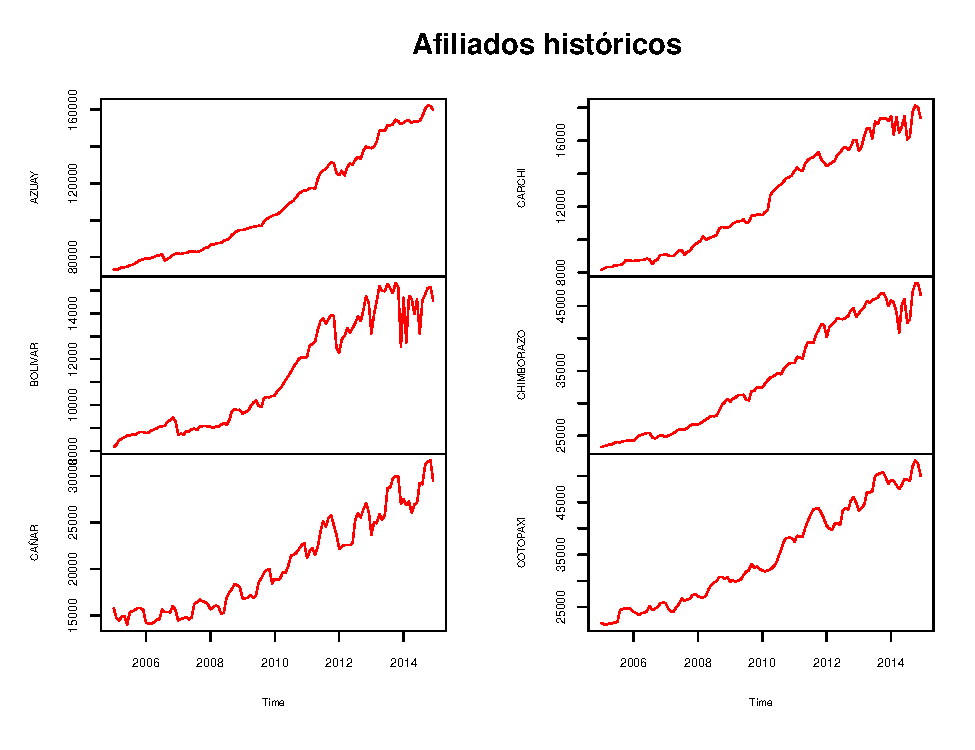
\includegraphics[width=\maxwidth]{figure/unnamed-chunk-1-1} 

}




{\centering 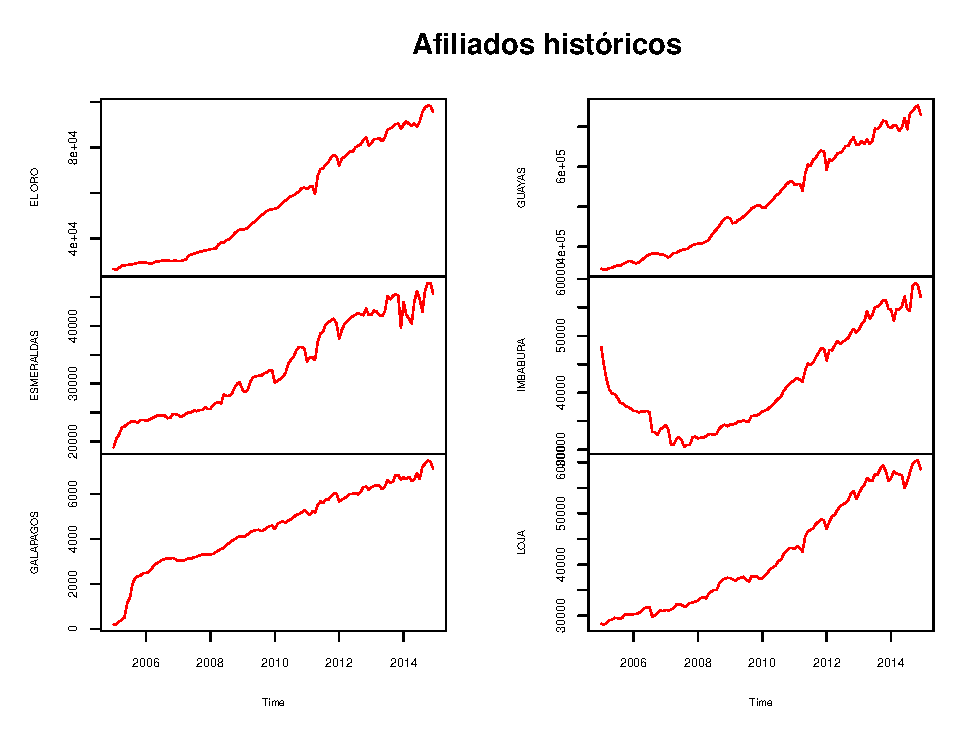
\includegraphics[width=\maxwidth]{figure/unnamed-chunk-1-2} 

}




{\centering 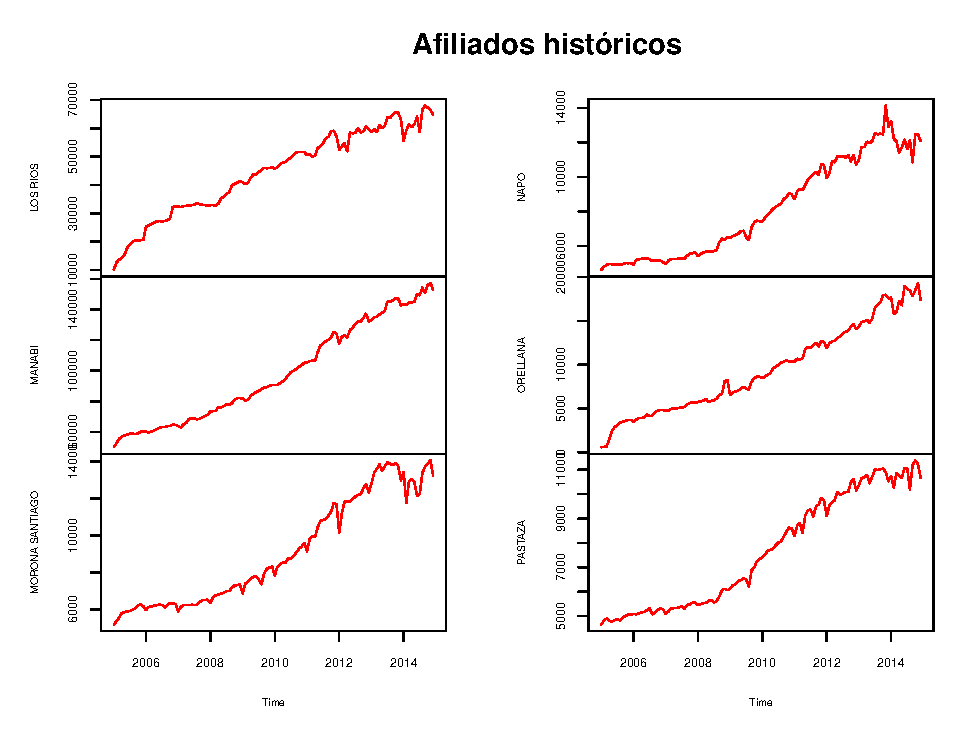
\includegraphics[width=\maxwidth]{figure/unnamed-chunk-1-3} 

}




{\centering 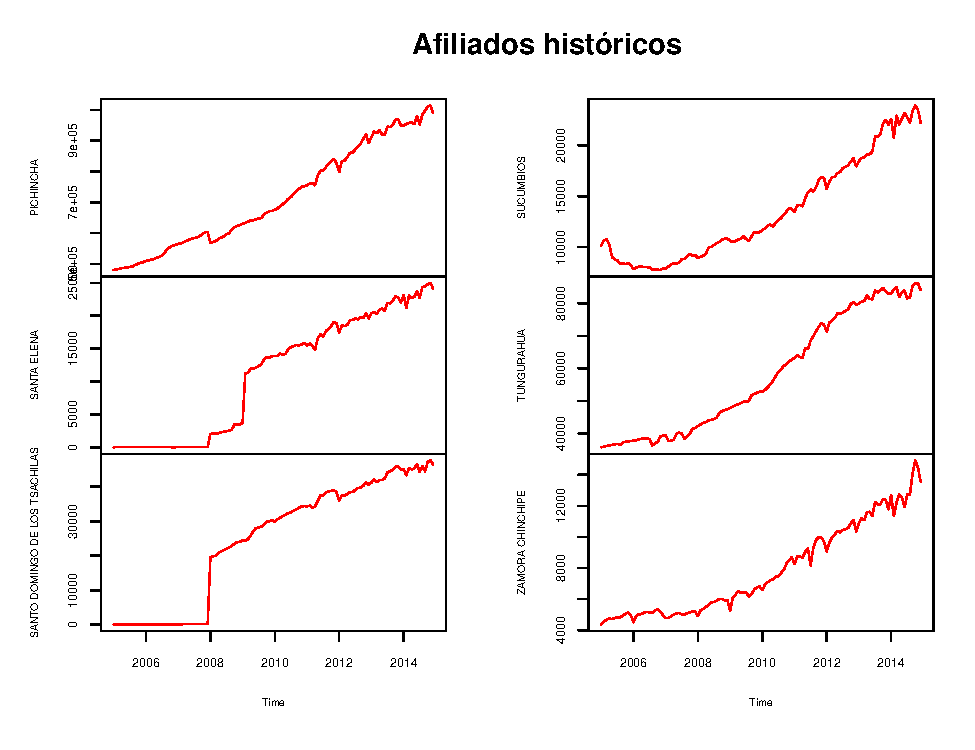
\includegraphics[width=\maxwidth]{figure/unnamed-chunk-1-4} 

}



\end{knitrout}

%Debido a la tendencia lineal que presentan las gráficas se procedió a diferenciar las mismas y a su vez obtener los correlogramas de la serie diferenciada:

Al observar las gráficas de las series se evidencia que las mismas no son estacionarias pues presentan una tendencia estocástica.\newline

La no estacionariedad se debe a la existencia de raíces unitarias en las series de afiliados, generalmente para obtener una serie estacionaria en media se procede a diferenciar la serie y seguido aplicar una prueba estadística que nos garantice la estacionariedad en varianza.\newline

Para el presente análisis implementaremos la prueba de estacionariedad de Kwiatkowski-Phillips-Schmidt-Shin (KPSS), la cual a diferencia de la prueba de raíz unitaria de Dickey Fuller, nos proporciona la prueba directa de la hipótesis nula de estacionariedad frente a la hipótesis alternativa de existencia de una raíz unitaria. La hipótesis nula y alternativa de la prueba KPSS es la siguiente:

\[\left\{\begin{tabular}{l}$H_0$: La serie es estacionaria\\ $H_1$: Existen raíces unitarias  \end{tabular}\right.\]


\subsection{Ajuste de afiliados Guayas}

\begin{knitrout}
\definecolor{shadecolor}{rgb}{0.969, 0.969, 0.969}\color{fgcolor}

{\centering 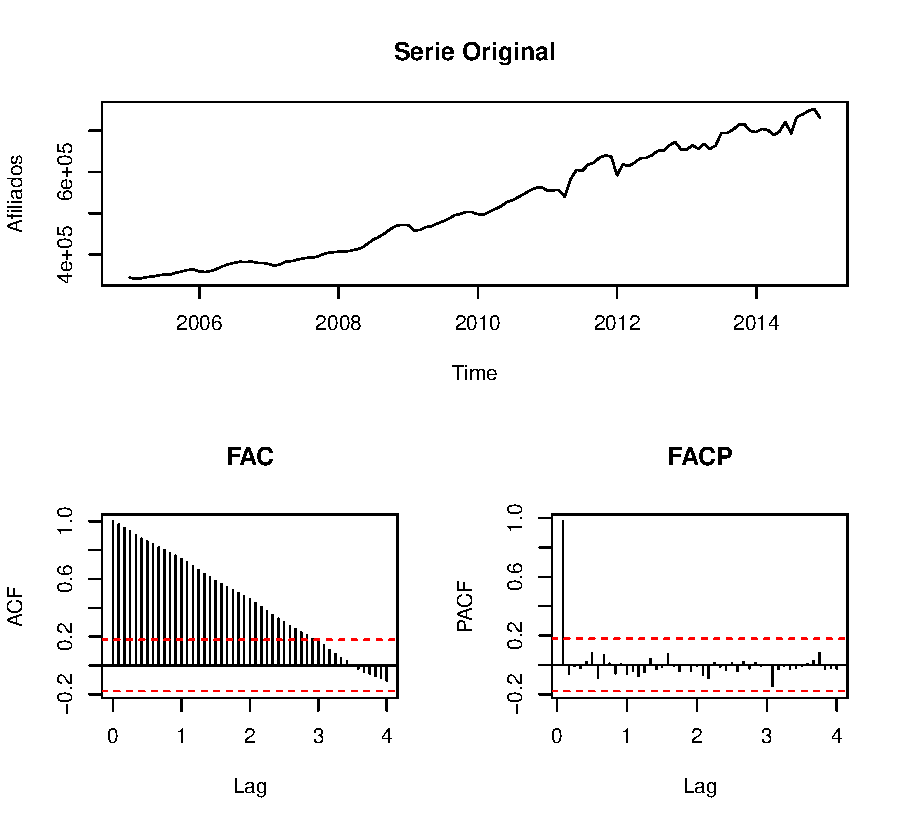
\includegraphics[width=\maxwidth]{figure/unnamed-chunk-2-1} 

}



\end{knitrout}

Los correlogramas muestran un decaimiento lento de la función ACF y un pico en el retardo 1 de la función PACF, esto muestra un comportamiento no estacionario y la necesidad de diferenciar la serie.

\begin{knitrout}
\definecolor{shadecolor}{rgb}{0.969, 0.969, 0.969}\color{fgcolor}\begin{kframe}
\begin{verbatim}
## 
## 	KPSS Test for Level Stationarity
## 
## data:  data[, 10]
## KPSS Level = 4.0757, Truncation lag parameter = 2, p-value = 0.01
\end{verbatim}
\end{kframe}
\end{knitrout}

Dado que el p-value de la prueba KPSS es menor al nivel de significancia 0.05, se rechaza la hipótesis nula. Esta prueba corrobora la existencia de raíces unitarias lo cual ocasionan la no estacionariedad.

\begin{knitrout}
\definecolor{shadecolor}{rgb}{0.969, 0.969, 0.969}\color{fgcolor}

{\centering 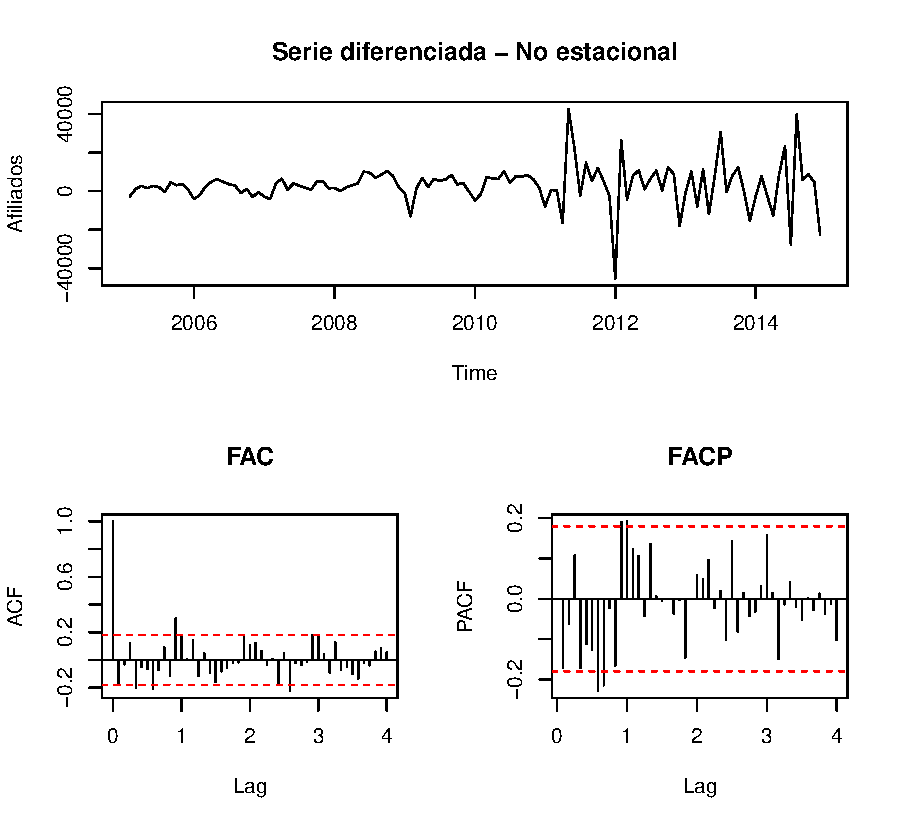
\includegraphics[width=\maxwidth]{figure/unnamed-chunk-4-1} 

}



\end{knitrout}

\begin{knitrout}
\definecolor{shadecolor}{rgb}{0.969, 0.969, 0.969}\color{fgcolor}\begin{kframe}
\begin{verbatim}
## 
## 	KPSS Test for Level Stationarity
## 
## data:  diff(data[, 10])
## KPSS Level = 0.094912, Truncation lag parameter = 2, p-value = 0.1
\end{verbatim}
\end{kframe}
\end{knitrout}

Observamos que el p-value de la prueba KPSS es superior al nivel de significancia 0.05, por lo cual aceptamos la hipótesis nula, es decir, la serie es estacionaria.\newline

Observamos que la función PACF de la serie diferenciada presenta picos en los retardos 12, 24, 36, 48 con decaimiento lento, lo cual nos conduce a la necesidad de diferenciación estacional de los datos.

\begin{knitrout}
\definecolor{shadecolor}{rgb}{0.969, 0.969, 0.969}\color{fgcolor}

{\centering 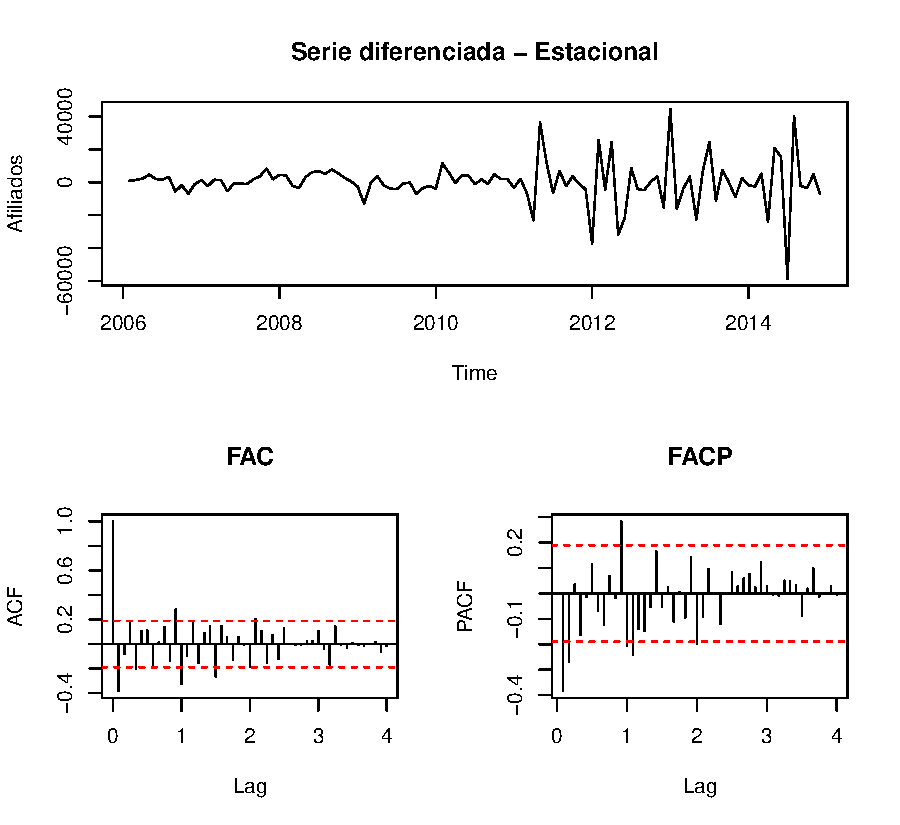
\includegraphics[width=\maxwidth]{figure/unnamed-chunk-6-1} 

}



\end{knitrout}

La función ACF presenta un pico en el retardo 12 y valores menores para los retardos 24, 36, 48. Por lo tanto, se sugieren los modelos MA estacional de orden 1 (Q=1). De igual manera los retardos no estacionales $h=1,2,\ldots, 11$ de la función PACF decaen, indicando que se debe ajustar un modelo  para el comportamiento no estacional de la serie, en principio tomamos $q=1$.\newline

Una vez identificado el modelo a ajustarse sobre la serie correspondiente al número de afiliados de la provincia de Guayas se procede al cálculo del mismo.

\begin{knitrout}
\definecolor{shadecolor}{rgb}{0.969, 0.969, 0.969}\color{fgcolor}\begin{kframe}
\begin{verbatim}
## Series: data[, 10] 
## ARIMA(0,1,1)(0,0,1)[12] with drift         
## 
## Coefficients:
##           ma1    sma1      drift
##       -0.2913  0.2949  3249.9255
## s.e.   0.0962  0.1032   821.4847
## 
## sigma^2 estimated as 98937829:  log likelihood=-1264.84
## AIC=2537.68   AICc=2538.03   BIC=2548.79
\end{verbatim}
\end{kframe}
\end{knitrout}

\begin{knitrout}
\definecolor{shadecolor}{rgb}{0.969, 0.969, 0.969}\color{fgcolor}
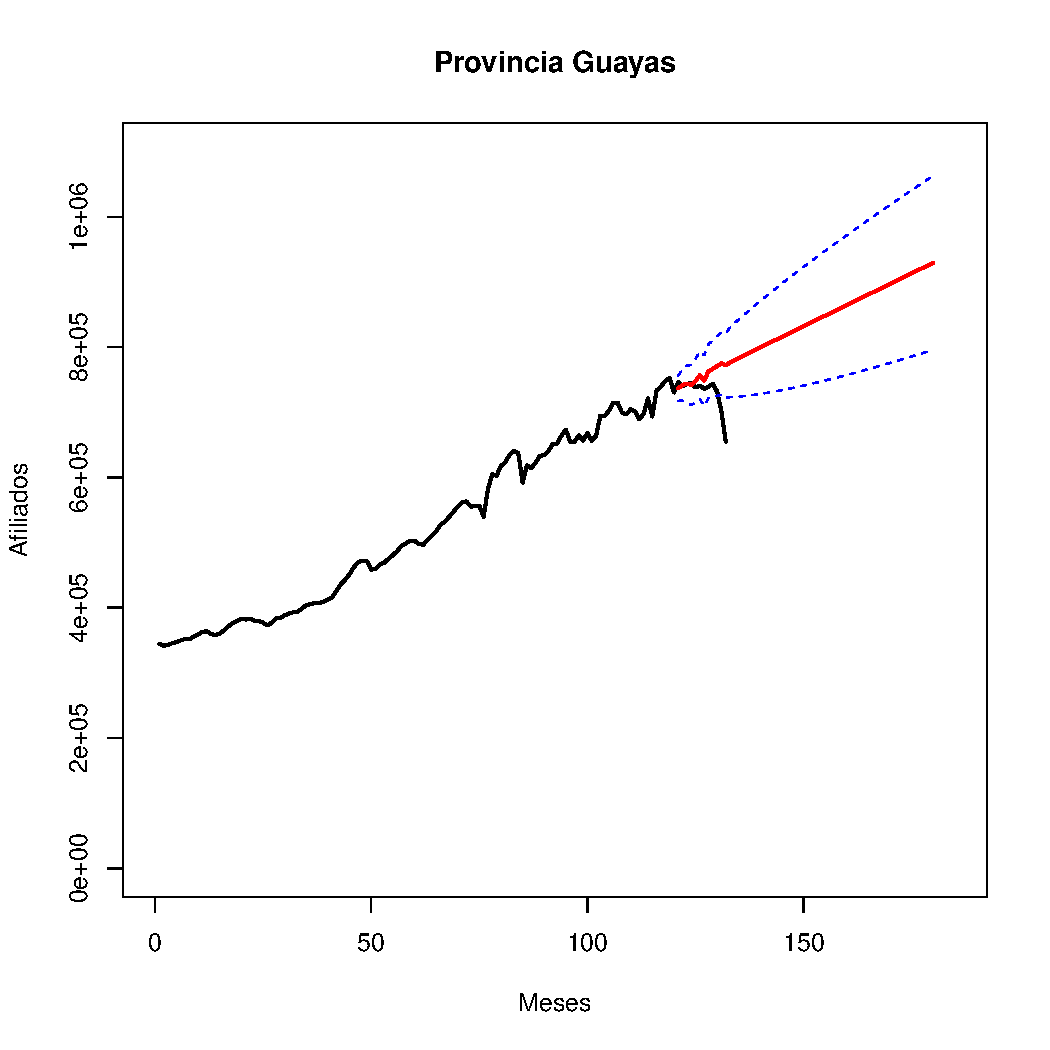
\includegraphics[width=\maxwidth]{figure/unnamed-chunk-8-1} 

\end{knitrout}

\subsection{Ajuste de afiliados Pichincha}

\begin{knitrout}
\definecolor{shadecolor}{rgb}{0.969, 0.969, 0.969}\color{fgcolor}

{\centering 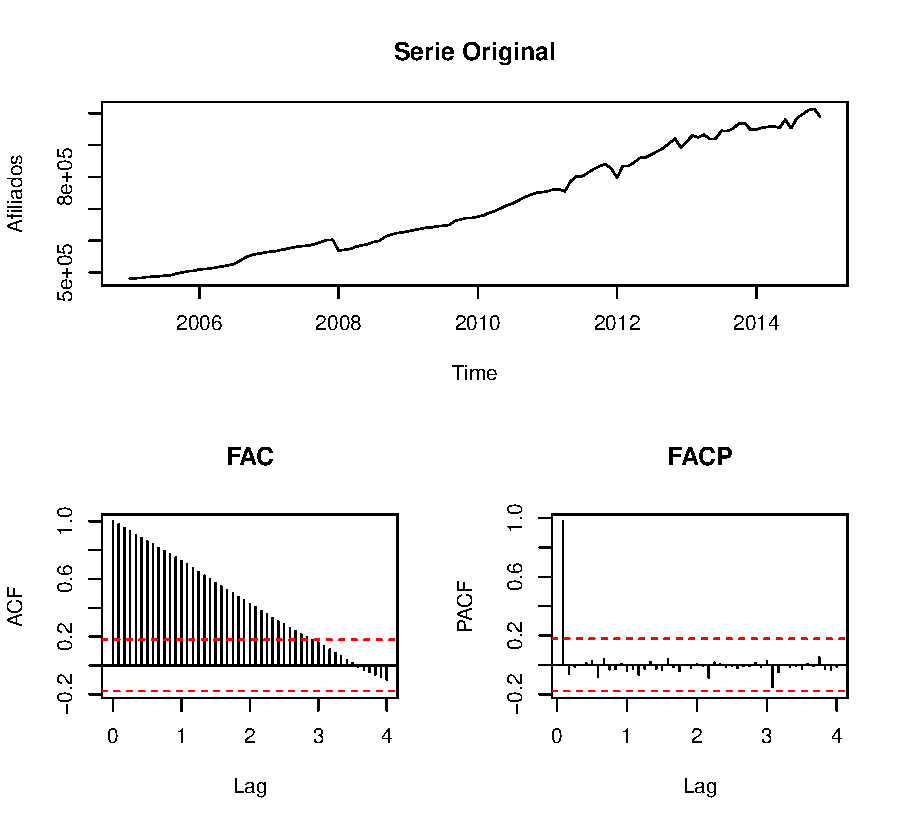
\includegraphics[width=\maxwidth]{figure/unnamed-chunk-9-1} 

}



\end{knitrout}

Los correlogramas muestran un decaimiento lento de la función ACF y un pico en el retardo 1 de la función PACF, lo cual implica que la serie tiene un comportamiento no estacionario y surge la necesidad de diferenciar la misma.

\begin{knitrout}
\definecolor{shadecolor}{rgb}{0.969, 0.969, 0.969}\color{fgcolor}\begin{kframe}
\begin{verbatim}
## 
## 	KPSS Test for Level Stationarity
## 
## data:  data[, 19]
## KPSS Level = 4.0451, Truncation lag parameter = 2, p-value = 0.01
\end{verbatim}
\end{kframe}
\end{knitrout}

La prueba KPSS corrobora el hecho que la serie es no estacionaria, pues el p-value es menor al nivel de significancia 0.05 lo cual implica  la existencia de raíces unitarias.

\begin{knitrout}
\definecolor{shadecolor}{rgb}{0.969, 0.969, 0.969}\color{fgcolor}

{\centering 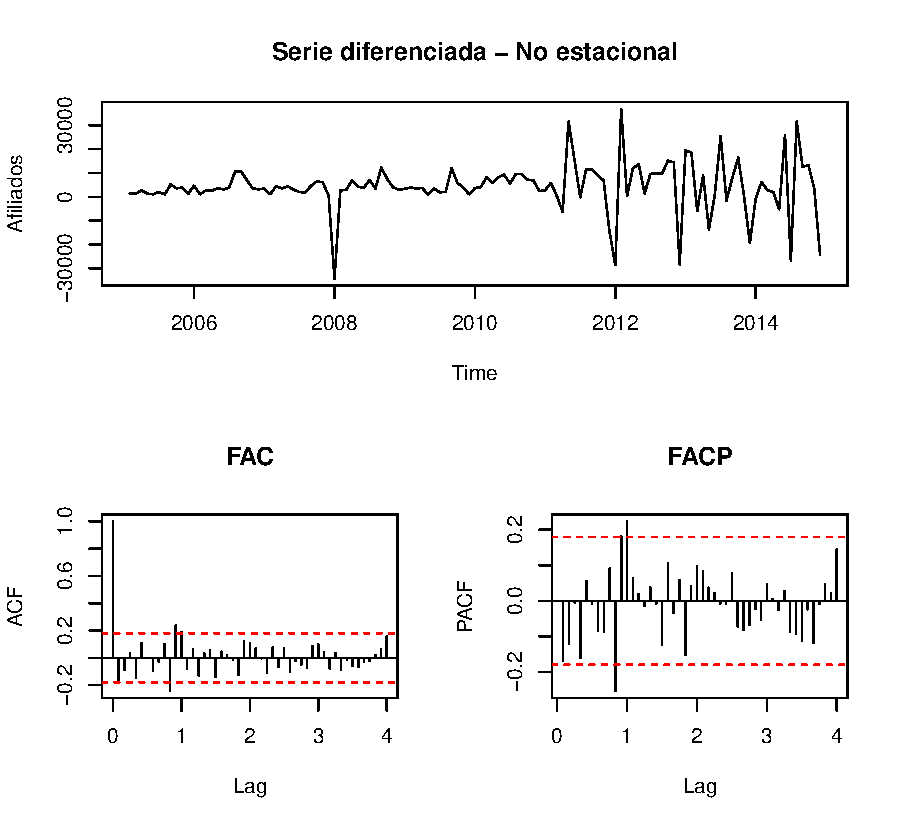
\includegraphics[width=\maxwidth]{figure/unnamed-chunk-11-1} 

}



\end{knitrout}

\begin{knitrout}
\definecolor{shadecolor}{rgb}{0.969, 0.969, 0.969}\color{fgcolor}\begin{kframe}
\begin{verbatim}
## 
## 	KPSS Test for Level Stationarity
## 
## data:  diff(data[, 19])
## KPSS Level = 0.14489, Truncation lag parameter = 2, p-value = 0.1
\end{verbatim}
\end{kframe}
\end{knitrout}

Observamos que el p-value de la prueba KPSS es superior al nivel de significancia 0.05, por lo cual aceptamos la hipótesis nula, es decir, la serie es estacionaria.\newline

Observamos que la función PACF de la serie diferenciada presenta picos en los retardos 12, 24, 36, 48 con decaimiento lento, lo cual nos conduce a la necesidad de diferenciación estacional de los datos.

\begin{knitrout}
\definecolor{shadecolor}{rgb}{0.969, 0.969, 0.969}\color{fgcolor}

{\centering 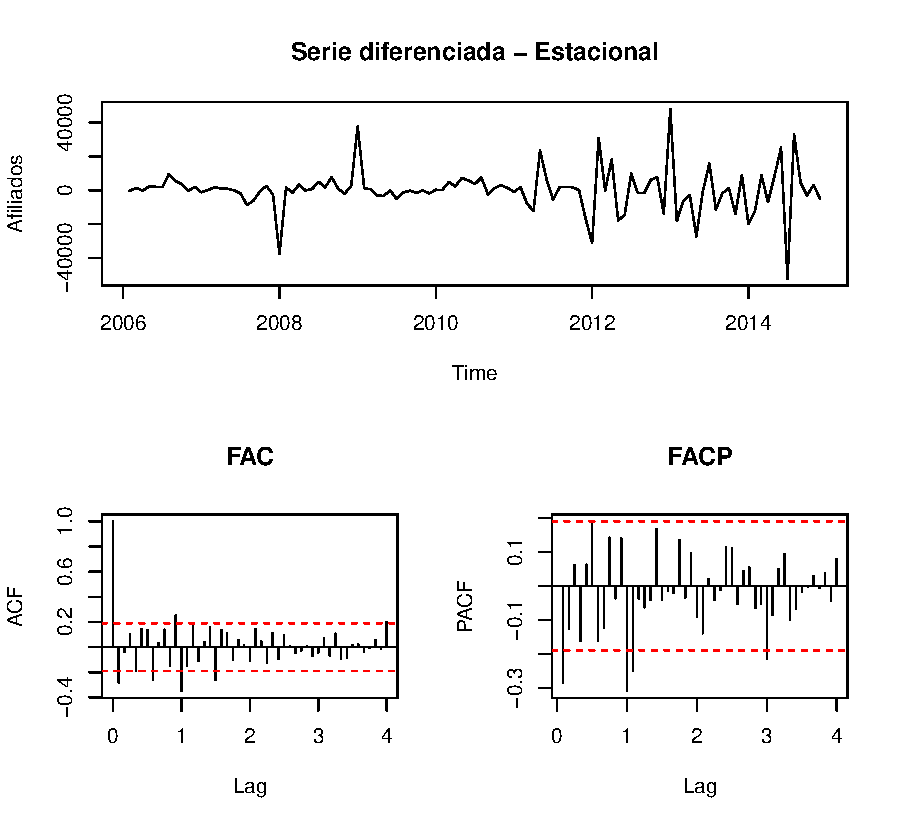
\includegraphics[width=\maxwidth]{figure/unnamed-chunk-13-1} 

}



\end{knitrout}


La función ACF presenta dos picos los retardo 12 y 13, mientras valores menores para los retardos 24, 25, 36, 37. Por lo tanto, se sugieren los modelos MA estacional de orden 2 (Q=2). De igual manera los retardos no estacionales $h=1,2,\ldots, 11$ de la función PACF decaen, indicando que se debe ajustar un modelo  para el comportamiento no estacional de la serie, en principio tomamos $p=1$ y $q=2$.\newline

Una vez identificado el modelo a ajustarse sobre la serie correspondiente al número de afiliados de la provincia de Pichincha se procede al cálculo del mismo.

\begin{knitrout}
\definecolor{shadecolor}{rgb}{0.969, 0.969, 0.969}\color{fgcolor}\begin{kframe}
\begin{verbatim}
## Series: data[, 19] 
## ARIMA(1,1,2)(0,0,2)[12] with drift         
## 
## Coefficients:
##           ar1     ma1      ma2    sma1    sma2      drift
##       -0.8265  0.6085  -0.3601  0.2209  0.1534  4313.3934
## s.e.   0.0708  0.1030   0.0948  0.1022  0.0890   786.5182
## 
## sigma^2 estimated as 88992256:  log likelihood=-1258.76
## AIC=2531.51   AICc=2532.52   BIC=2550.97
\end{verbatim}
\end{kframe}
\end{knitrout}

\begin{knitrout}
\definecolor{shadecolor}{rgb}{0.969, 0.969, 0.969}\color{fgcolor}
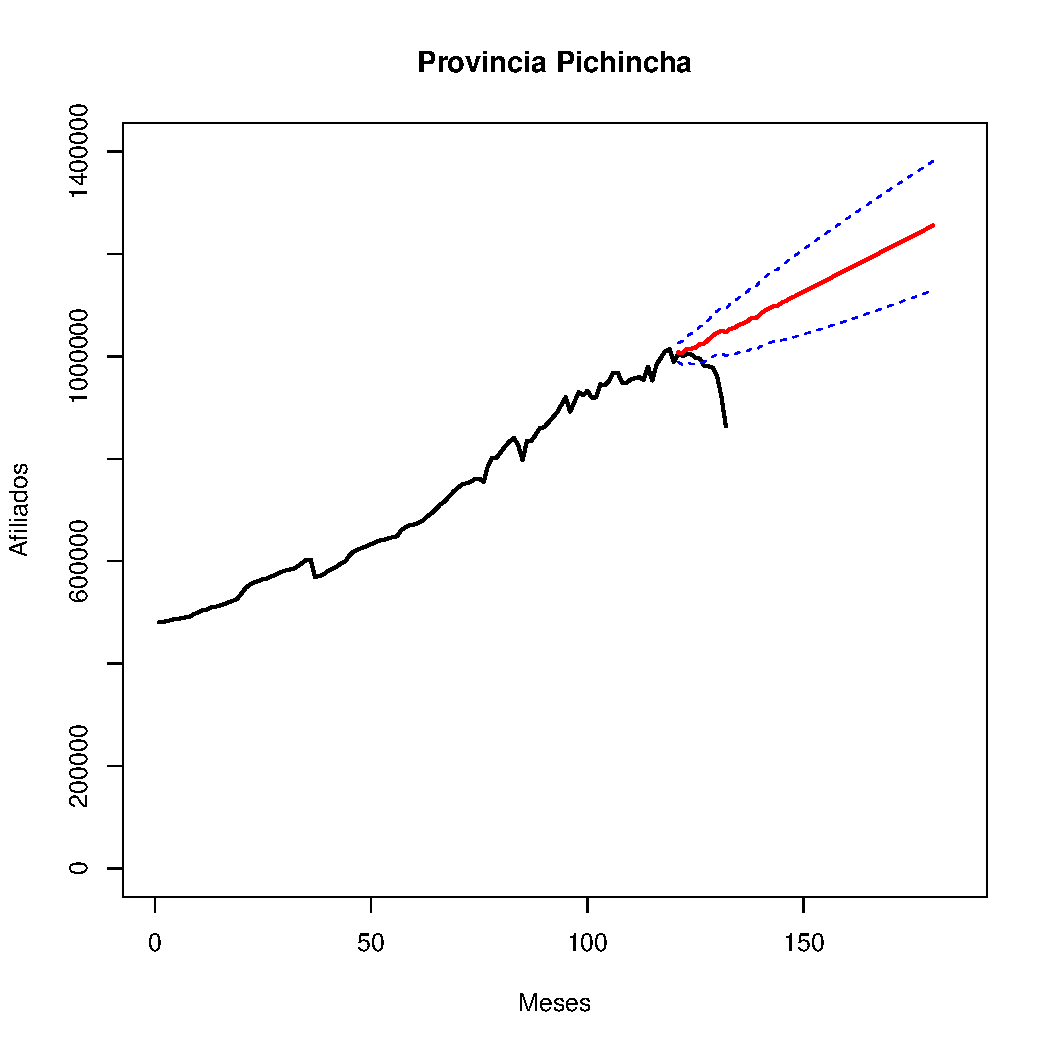
\includegraphics[width=\maxwidth]{figure/unnamed-chunk-15-1} 

\end{knitrout}

\subsection{Ajuste de afiliados del resto de provincias}

Una vez detallada la metodología a emplearse en la proyección del número de afiliados, se presentan los resultados obtenidos:

\begin{knitrout}
\definecolor{shadecolor}{rgb}{0.969, 0.969, 0.969}\color{fgcolor}

{\centering 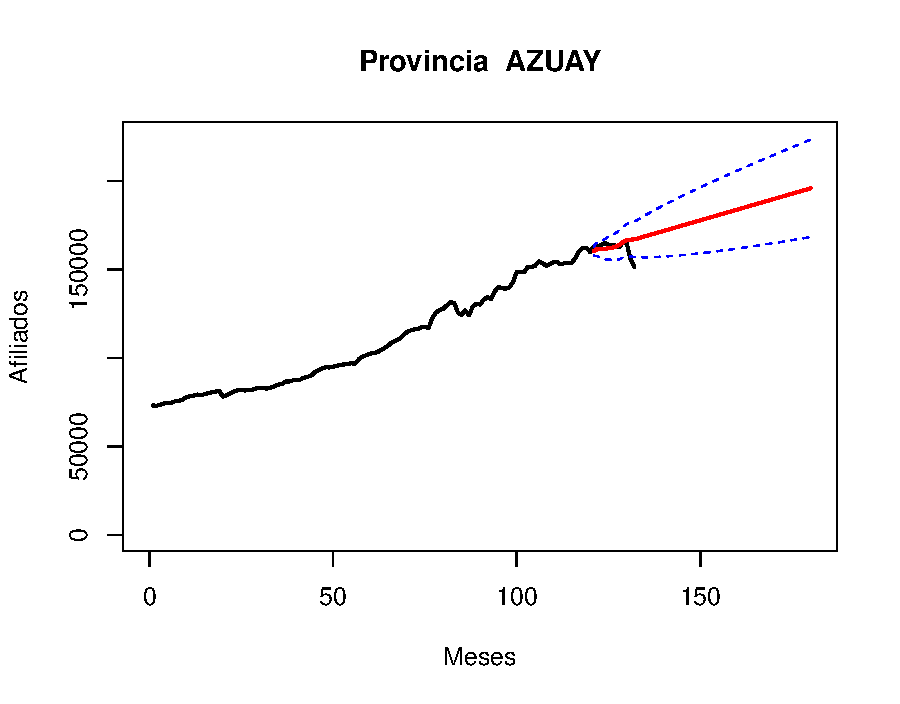
\includegraphics[width=\maxwidth]{figure/unnamed-chunk-16-1} 

}


\begin{kframe}\begin{verbatim}
## Series: data[, i] 
## ARIMA(2,1,2)(0,0,1)[12] with drift         
## 
## Coefficients:
##           ar1      ar2     ma1     ma2    sma1     drift
##       -1.3127  -0.7876  1.5596  0.8976  0.2793  600.9012
## s.e.   0.1199   0.1125  0.0966  0.1206  0.1167  163.7569
## 
## sigma^2 estimated as 1750671:  log likelihood=-1024.2
## AIC=2047.78   AICc=2048.79   BIC=2067.23
\end{verbatim}
\end{kframe}

{\centering 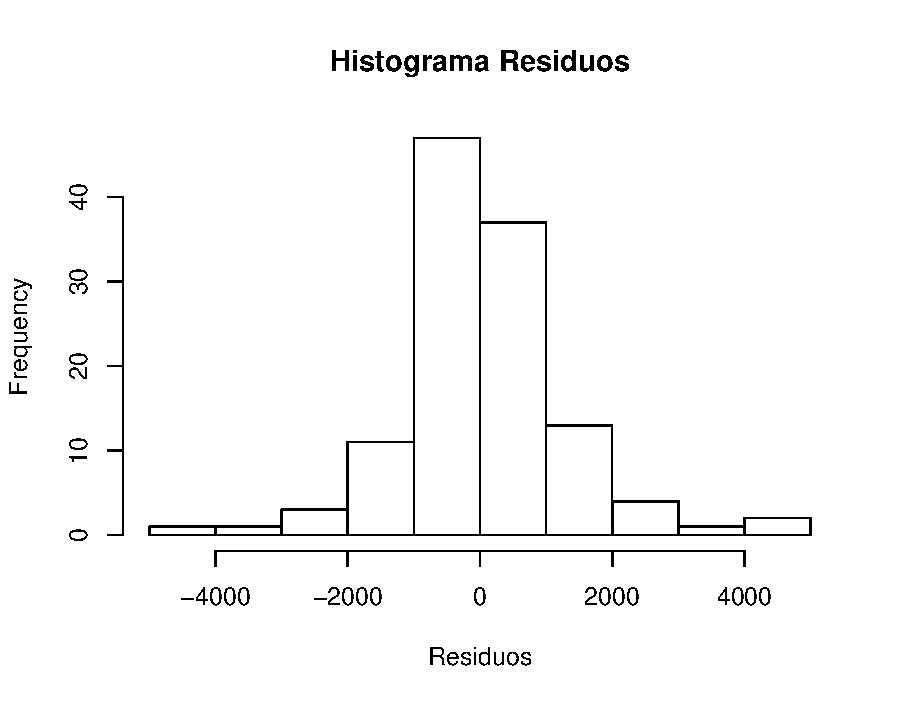
\includegraphics[width=\maxwidth]{figure/unnamed-chunk-16-2} 

}




{\centering 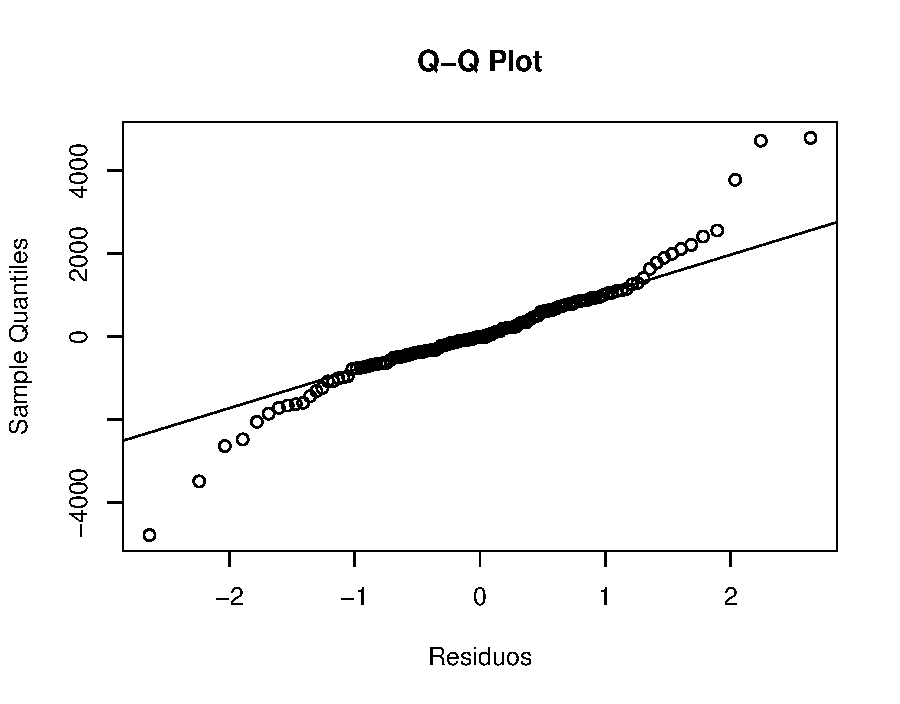
\includegraphics[width=\maxwidth]{figure/unnamed-chunk-16-3} 

}




{\centering 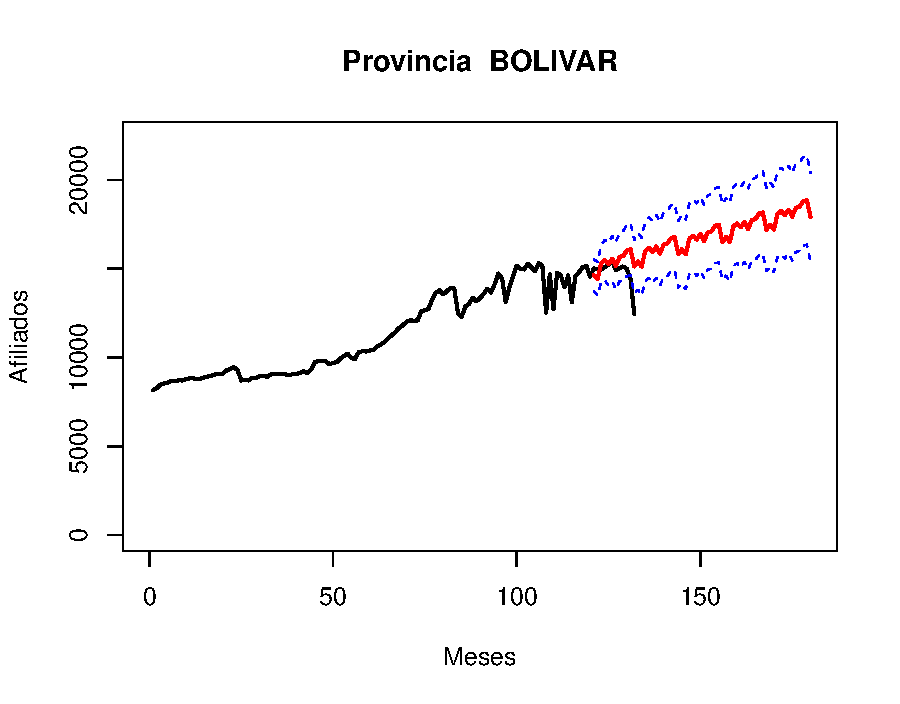
\includegraphics[width=\maxwidth]{figure/unnamed-chunk-16-4} 

}


\begin{kframe}\begin{verbatim}
## Series: data[, i] 
## ARIMA(1,0,2)(0,1,1)[12] with drift         
## 
## Coefficients:
##          ar1      ma1     ma2     sma1    drift
##       0.9370  -0.6243  0.2405  -0.6556  57.7468
## s.e.  0.0402   0.1011  0.0900   0.1059  13.4978
## 
## sigma^2 estimated as 207452:  log likelihood=-818.15
## AIC=1648.3   AICc=1649.13   BIC=1664.39
\end{verbatim}
\end{kframe}

{\centering 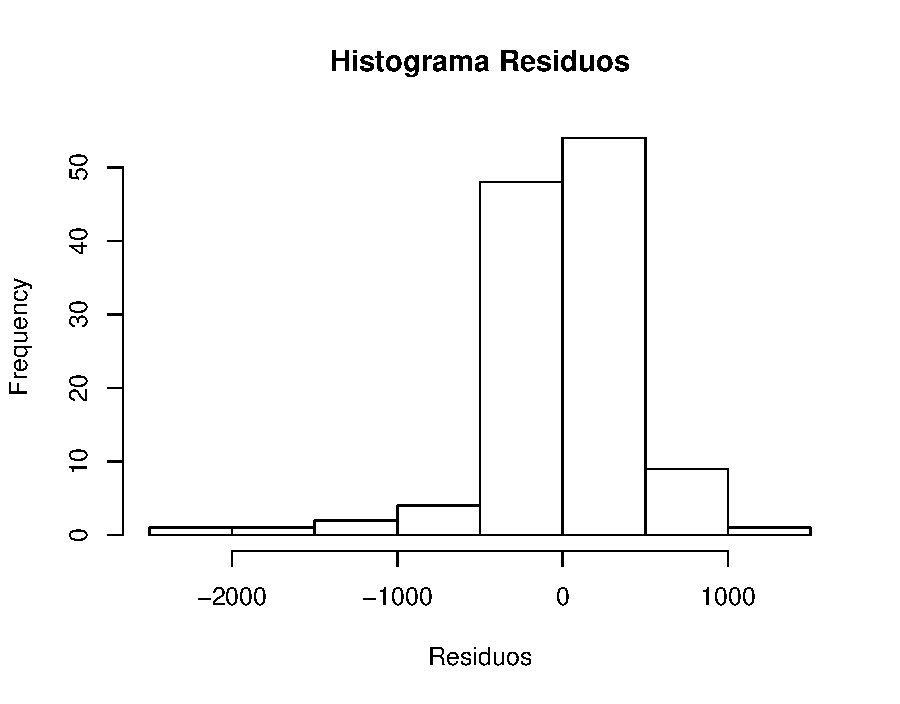
\includegraphics[width=\maxwidth]{figure/unnamed-chunk-16-5} 

}




{\centering 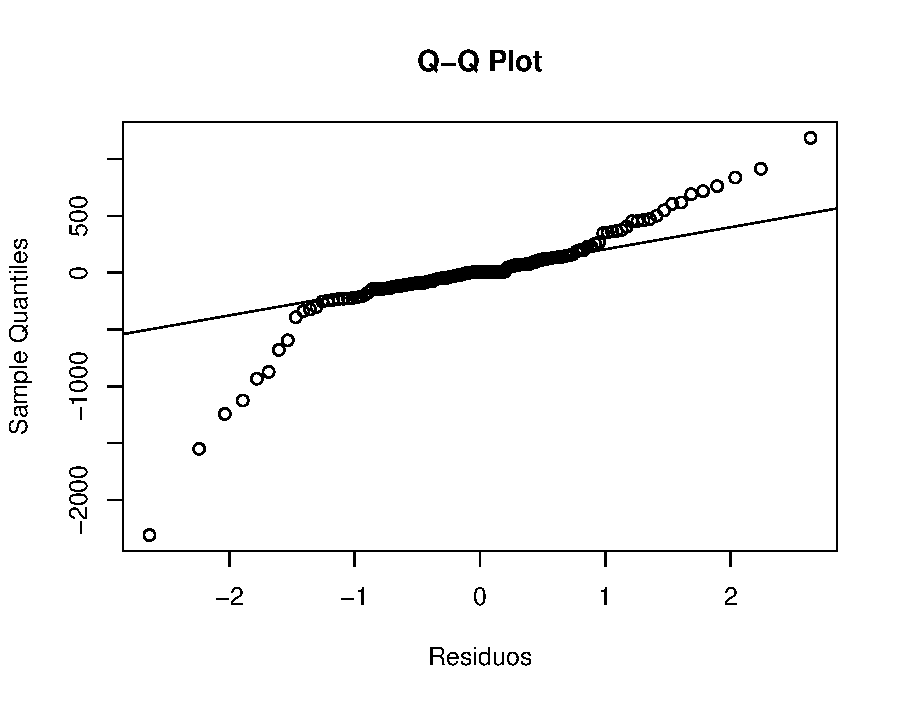
\includegraphics[width=\maxwidth]{figure/unnamed-chunk-16-6} 

}




{\centering 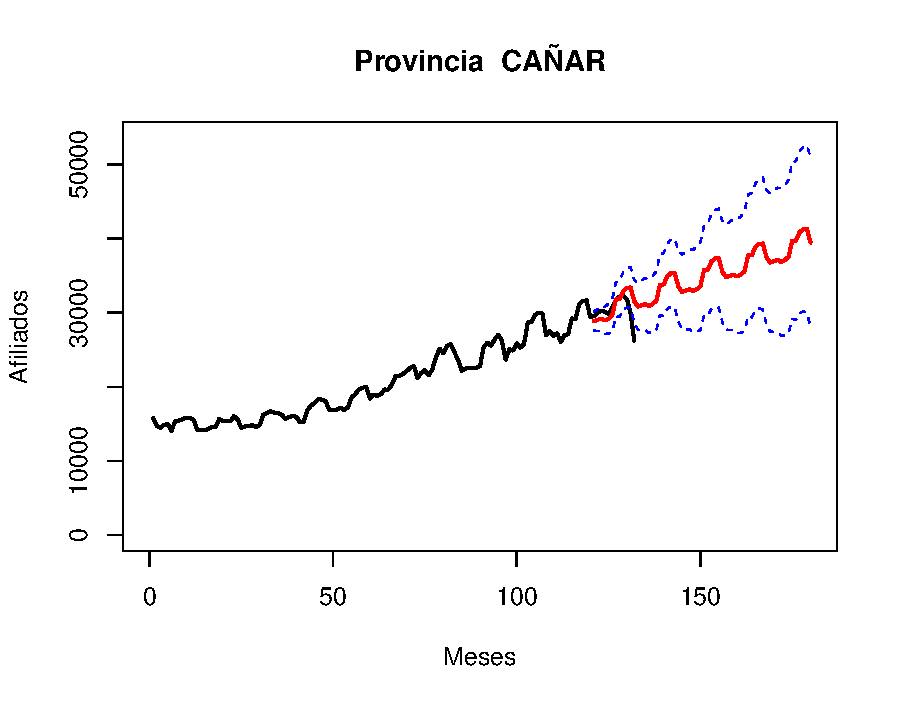
\includegraphics[width=\maxwidth]{figure/unnamed-chunk-16-7} 

}


\begin{kframe}\begin{verbatim}
## Series: data[, i] 
## ARIMA(1,1,1)(0,1,1)[12]                    
## 
## Coefficients:
##          ar1      ma1     sma1
##       0.0120  -0.3981  -0.6018
## s.e.  0.2495   0.2297   0.0915
## 
## sigma^2 estimated as 420574:  log likelihood=-847.4
## AIC=1702.8   AICc=1703.19   BIC=1713.49
\end{verbatim}
\end{kframe}

{\centering 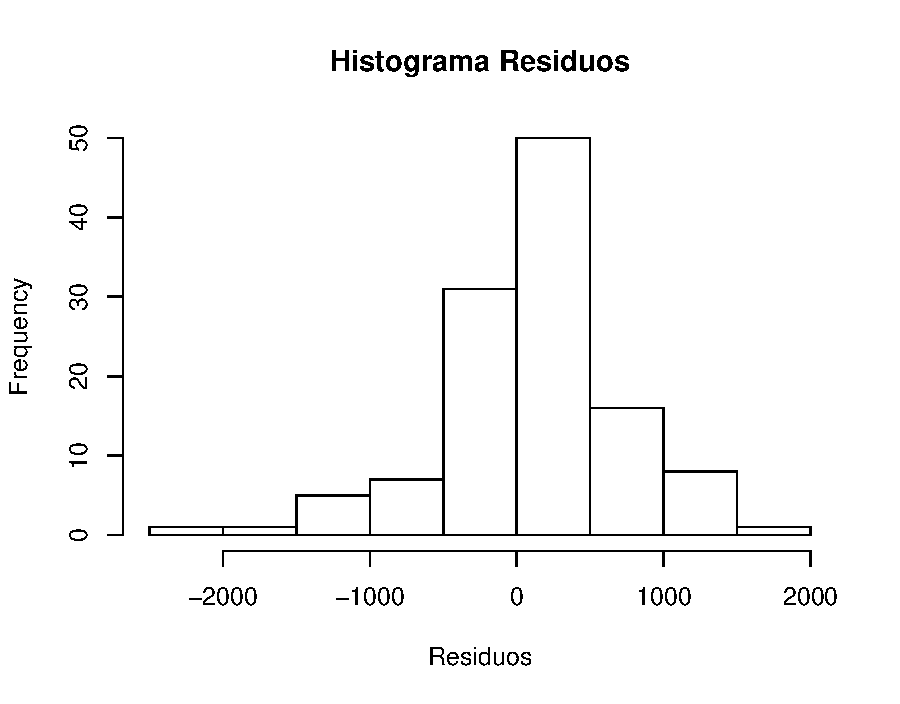
\includegraphics[width=\maxwidth]{figure/unnamed-chunk-16-8} 

}




{\centering 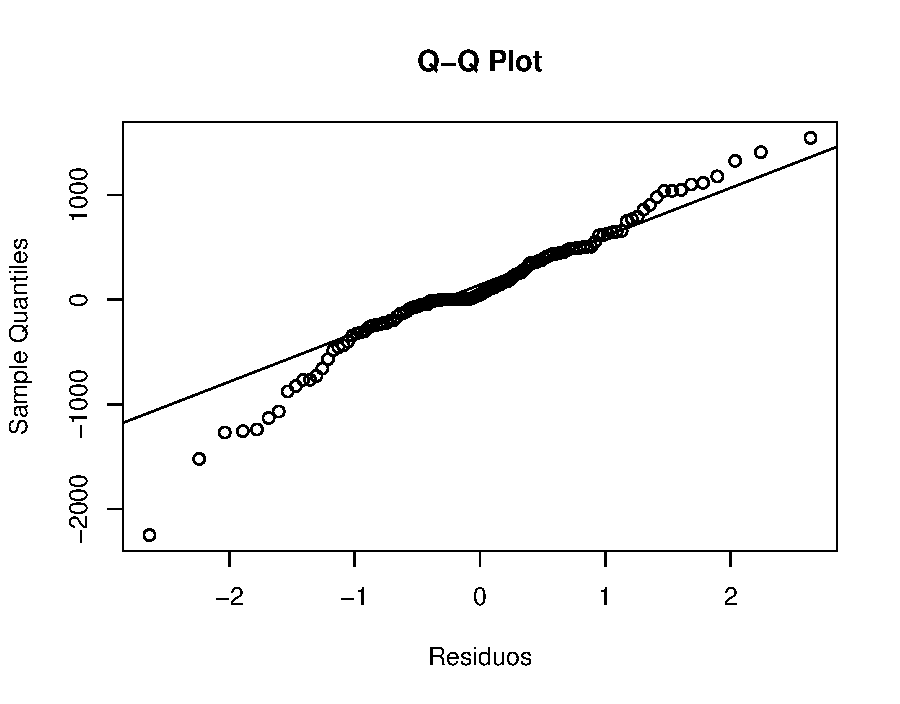
\includegraphics[width=\maxwidth]{figure/unnamed-chunk-16-9} 

}




{\centering 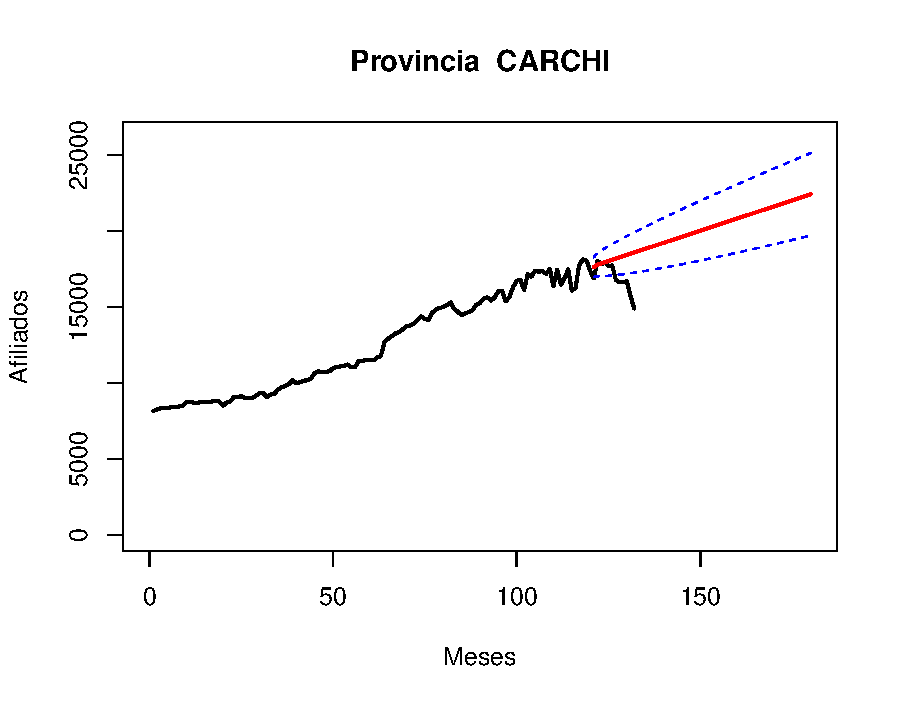
\includegraphics[width=\maxwidth]{figure/unnamed-chunk-16-10} 

}


\begin{kframe}\begin{verbatim}
## Series: data[, i] 
## ARIMA(0,1,2) with drift         
## 
## Coefficients:
##           ma1      ma2    drift
##       -0.3281  -0.1399  79.6781
## s.e.   0.0916   0.0897  16.1169
## 
## sigma^2 estimated as 107074:  log likelihood=-858.04
## AIC=1724.08   AICc=1724.43   BIC=1735.19
\end{verbatim}
\end{kframe}

{\centering 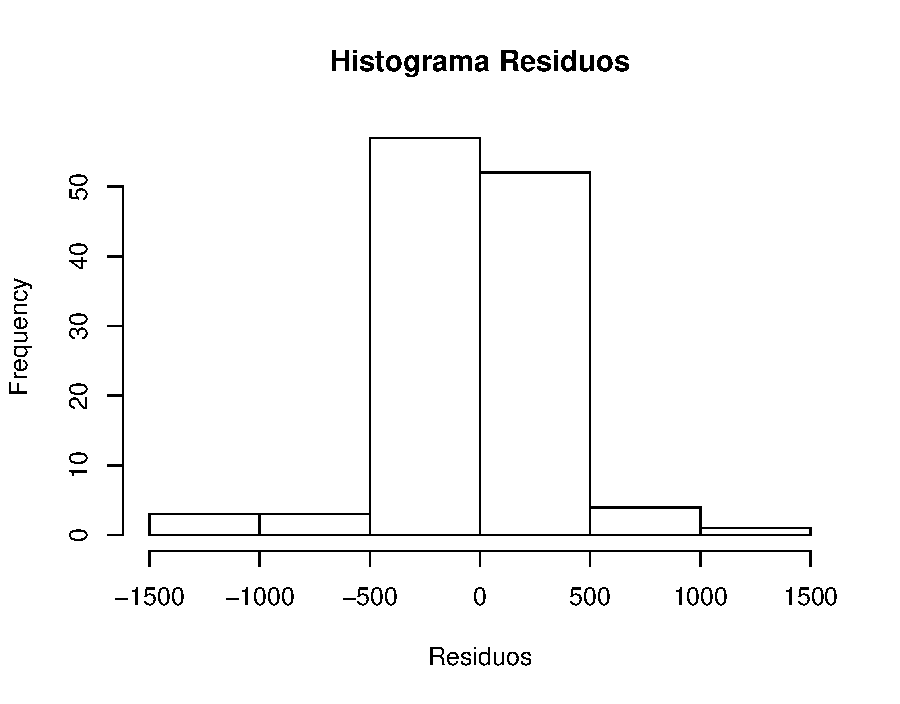
\includegraphics[width=\maxwidth]{figure/unnamed-chunk-16-11} 

}




{\centering 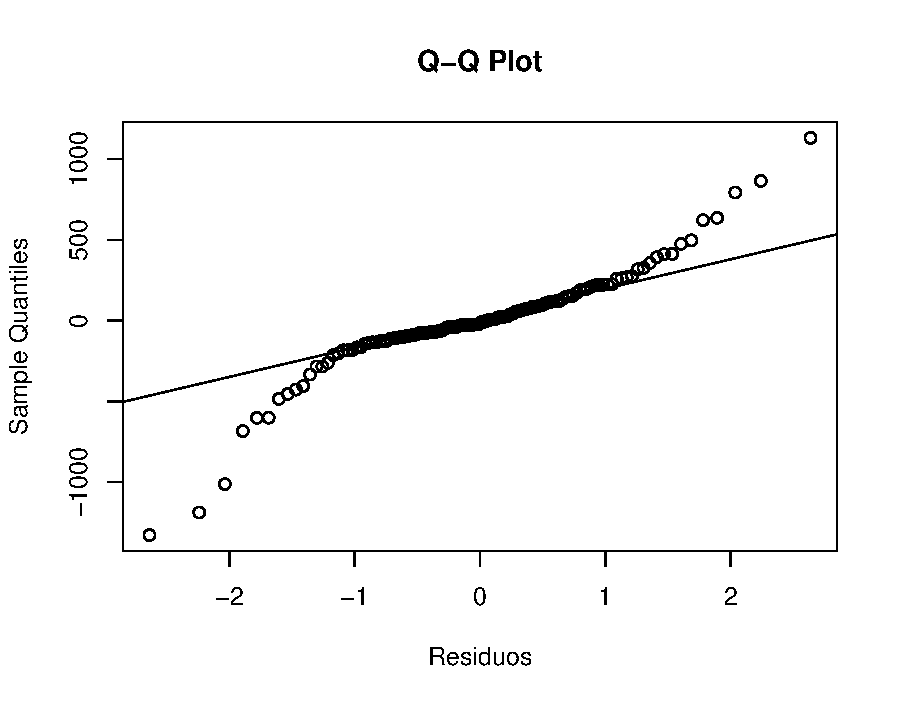
\includegraphics[width=\maxwidth]{figure/unnamed-chunk-16-12} 

}




{\centering 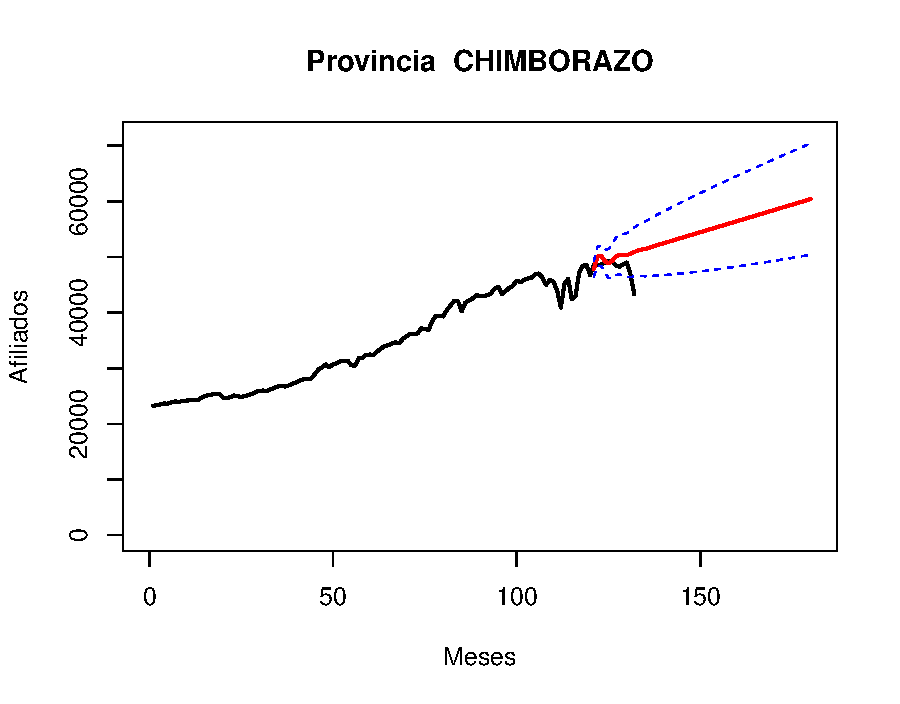
\includegraphics[width=\maxwidth]{figure/unnamed-chunk-16-13} 

}


\begin{kframe}\begin{verbatim}
## Series: data[, i] 
## ARIMA(2,1,3) with drift         
## 
## Coefficients:
##          ar1      ar2      ma1     ma2     ma3     drift
##       0.5599  -0.5733  -0.7919  0.2698  0.4577  198.3843
## s.e.  0.1072   0.1027   0.1032  0.1330  0.0923   59.7068
## 
## sigma^2 estimated as 514123:  log likelihood=-951.29
## AIC=1902.95   AICc=1903.95   BIC=1922.4
\end{verbatim}
\end{kframe}

{\centering 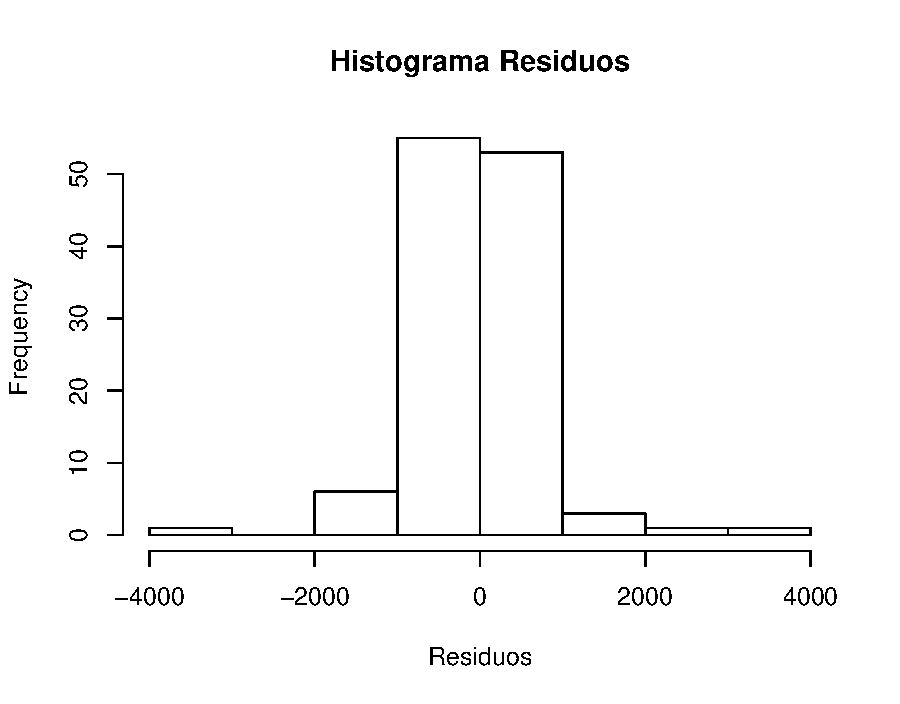
\includegraphics[width=\maxwidth]{figure/unnamed-chunk-16-14} 

}




{\centering 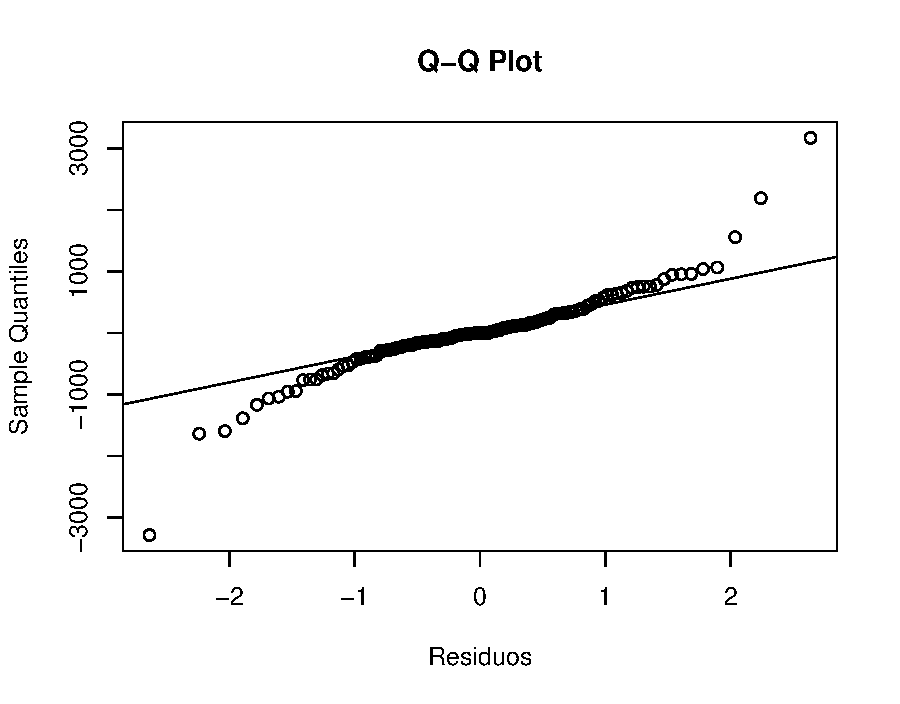
\includegraphics[width=\maxwidth]{figure/unnamed-chunk-16-15} 

}




{\centering 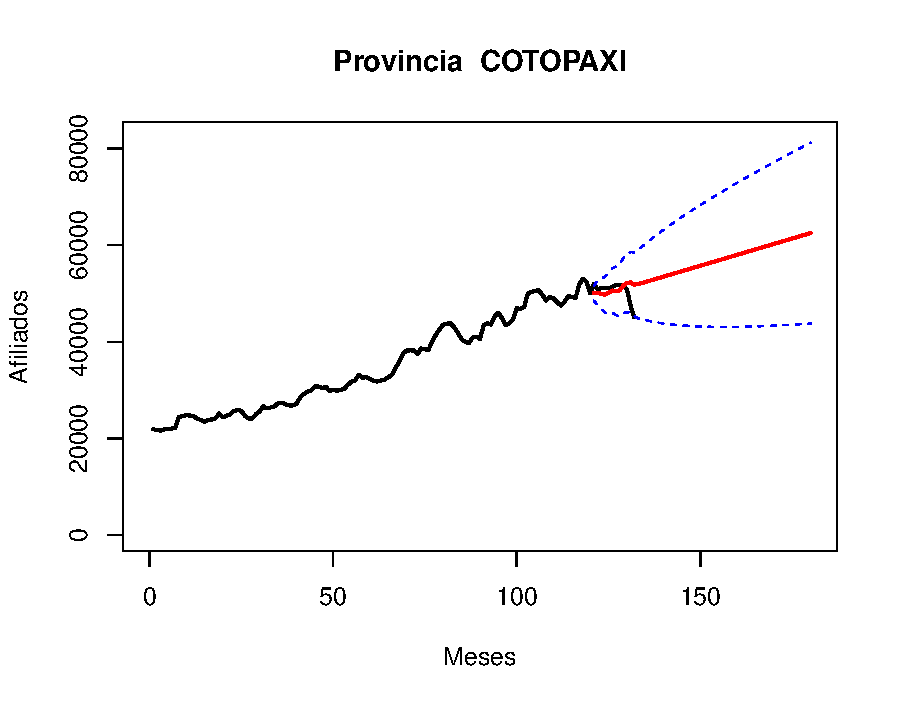
\includegraphics[width=\maxwidth]{figure/unnamed-chunk-16-16} 

}


\begin{kframe}\begin{verbatim}
## Series: data[, i] 
## ARIMA(0,1,1)(0,0,1)[12] with drift         
## 
## Coefficients:
##          ma1    sma1     drift
##       0.2365  0.3074  225.2014
## s.e.  0.0981  0.1050  115.3807
## 
## sigma^2 estimated as 636452:  log likelihood=-964.62
## AIC=1937.23   AICc=1937.58   BIC=1948.35
\end{verbatim}
\end{kframe}

{\centering 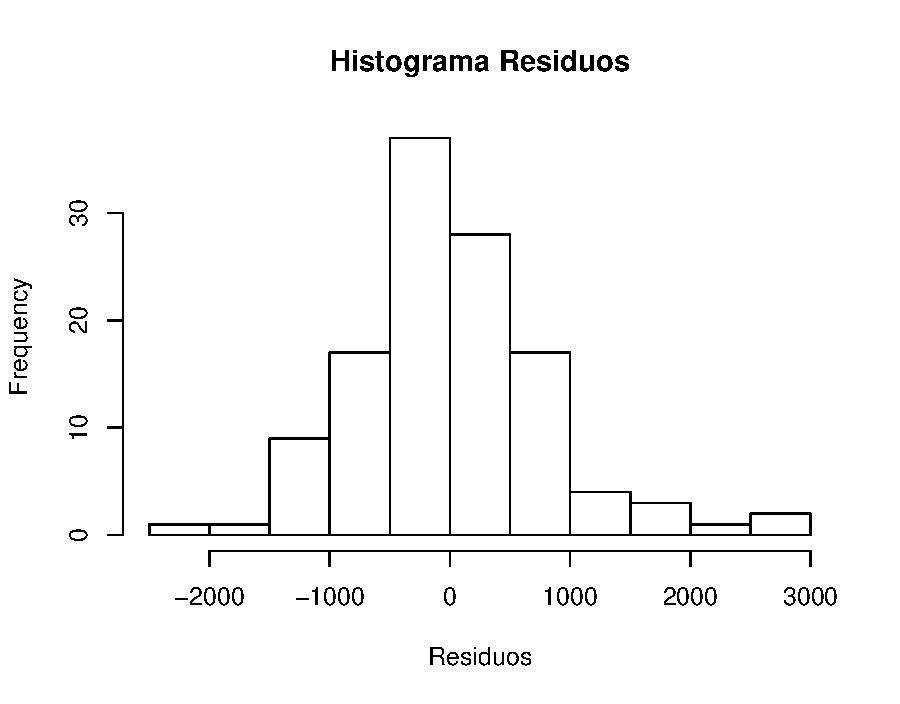
\includegraphics[width=\maxwidth]{figure/unnamed-chunk-16-17} 

}




{\centering 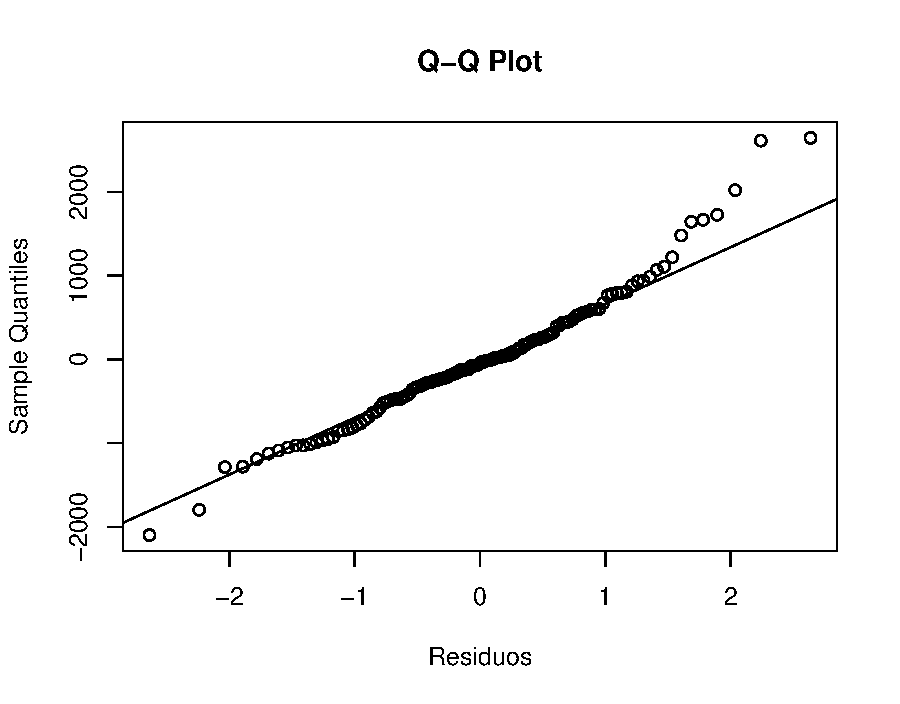
\includegraphics[width=\maxwidth]{figure/unnamed-chunk-16-18} 

}




{\centering 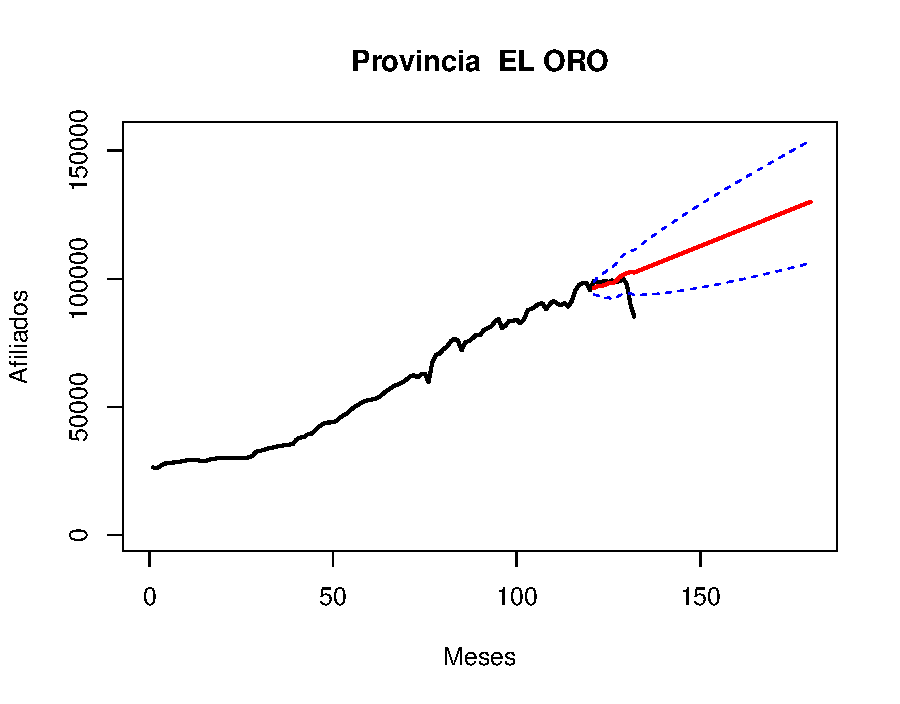
\includegraphics[width=\maxwidth]{figure/unnamed-chunk-16-19} 

}


\begin{kframe}\begin{verbatim}
## Series: data[, i] 
## ARIMA(0,1,0)(0,0,1)[12] with drift         
## 
## Coefficients:
##         sma1     drift
##       0.2749  575.2182
## s.e.  0.0876  147.2591
## 
## sigma^2 estimated as 1656548:  log likelihood=-1021.38
## AIC=2048.76   AICc=2048.97   BIC=2057.1
\end{verbatim}
\end{kframe}

{\centering 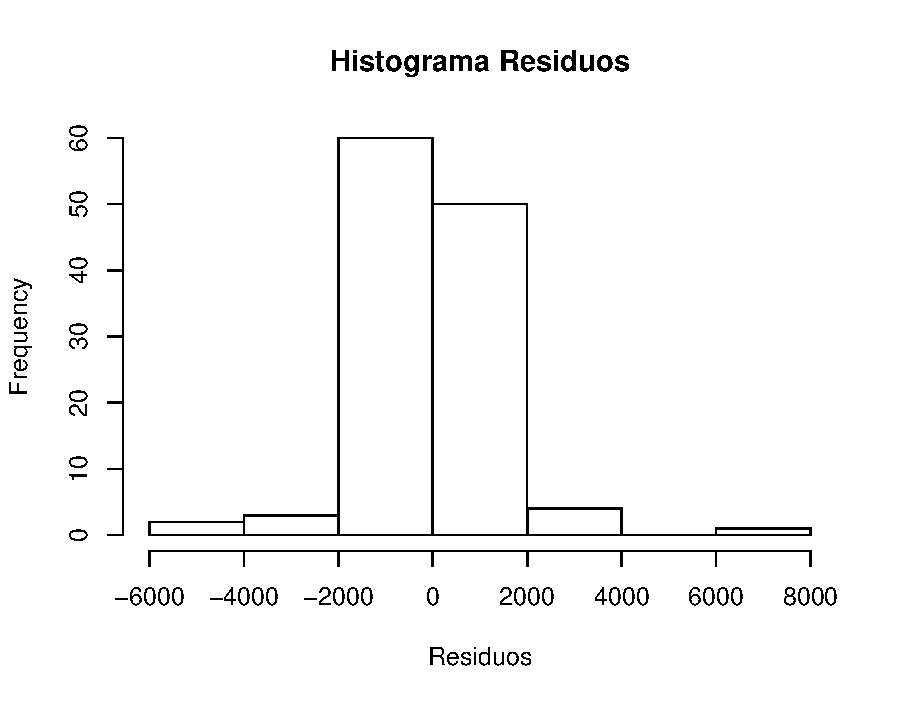
\includegraphics[width=\maxwidth]{figure/unnamed-chunk-16-20} 

}




{\centering 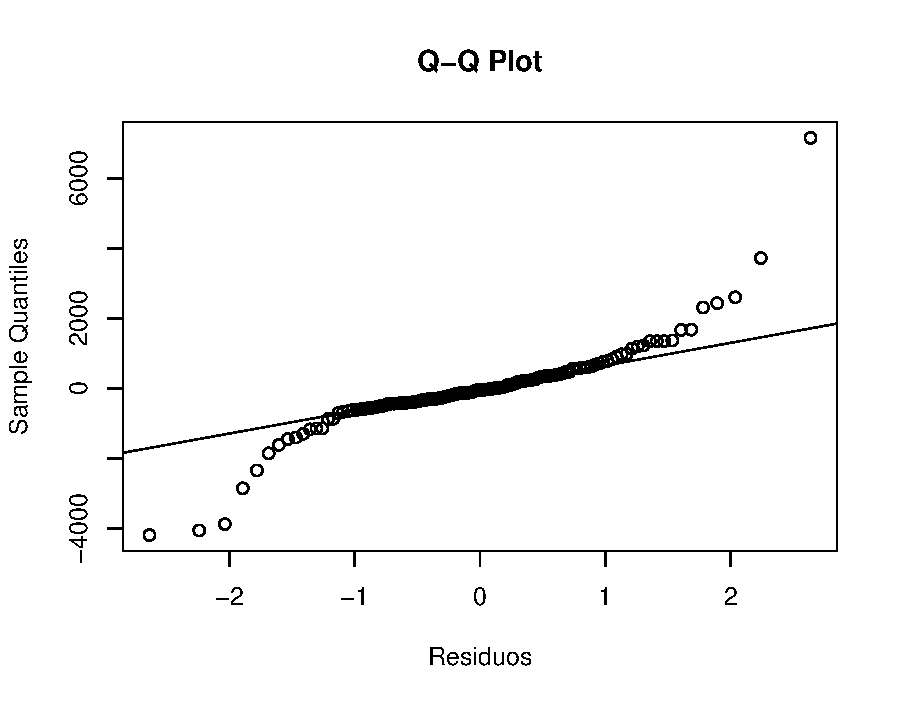
\includegraphics[width=\maxwidth]{figure/unnamed-chunk-16-21} 

}




{\centering 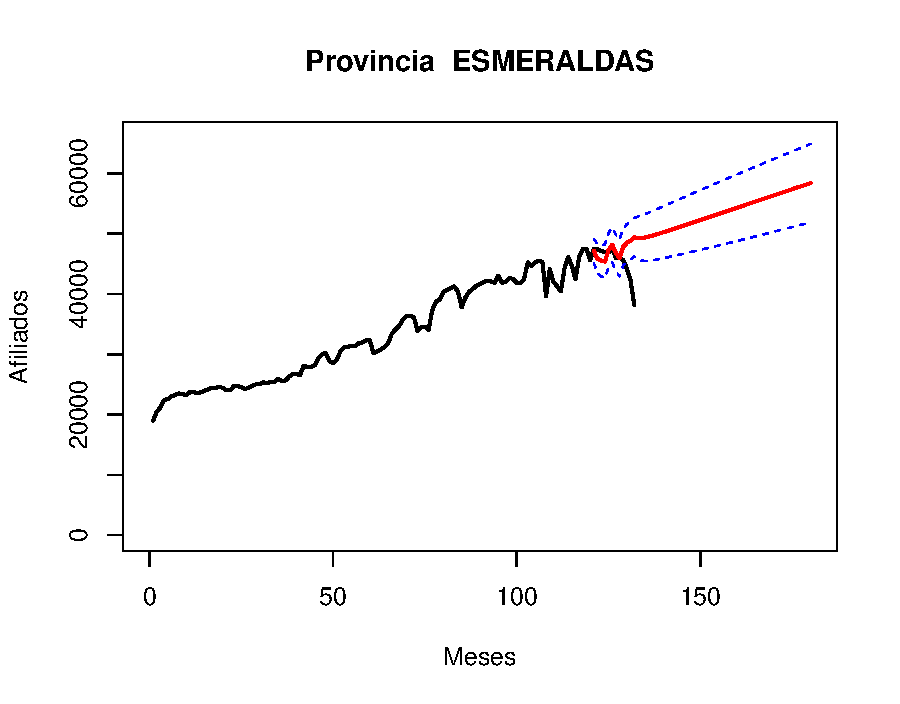
\includegraphics[width=\maxwidth]{figure/unnamed-chunk-16-22} 

}


\begin{kframe}\begin{verbatim}
## Series: data[, i] 
## ARIMA(1,1,1)(0,0,1)[12] with drift         
## 
## Coefficients:
##          ar1      ma1    sma1     drift
##       0.5797  -0.8943  0.5114  203.5063
## s.e.  0.0870   0.0558  0.1058   37.0427
## 
## sigma^2 estimated as 1063292:  log likelihood=-994.53
## AIC=1984.9   AICc=1985.43   BIC=1998.79
\end{verbatim}
\end{kframe}

{\centering 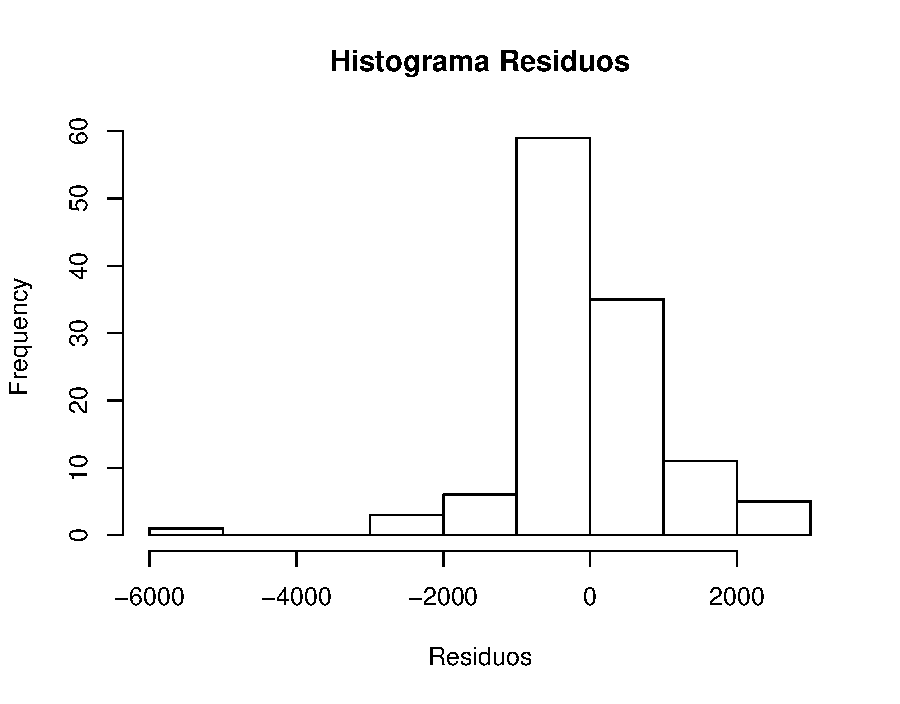
\includegraphics[width=\maxwidth]{figure/unnamed-chunk-16-23} 

}




{\centering 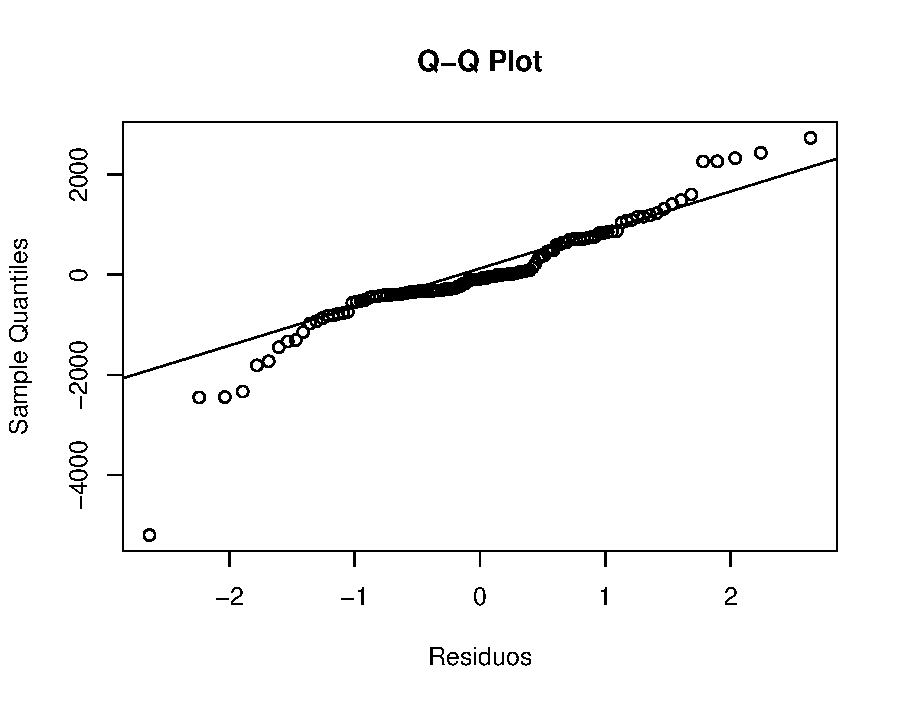
\includegraphics[width=\maxwidth]{figure/unnamed-chunk-16-24} 

}




{\centering 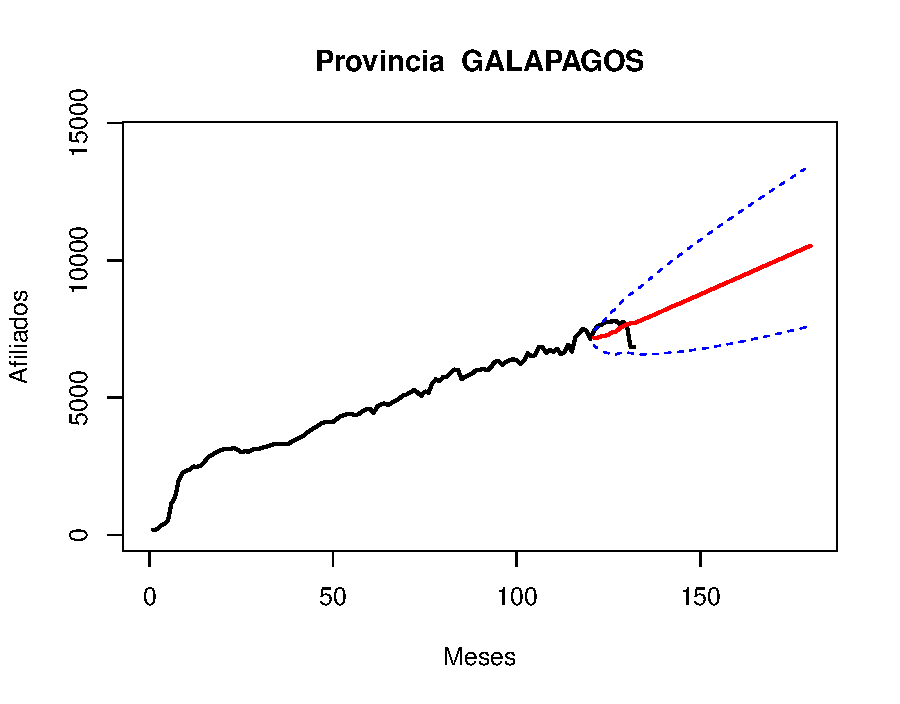
\includegraphics[width=\maxwidth]{figure/unnamed-chunk-16-25} 

}


\begin{kframe}\begin{verbatim}
## Series: data[, i] 
## ARIMA(2,1,1)(1,0,0)[12] with drift         
## 
## Coefficients:
##          ar1     ar2      ma1    sar1    drift
##       0.3235  0.1156  -0.2933  0.1298  59.1207
## s.e.  0.4523  0.0998   0.4543  0.1274  18.0832
## 
## sigma^2 estimated as 19056:  log likelihood=-755.35
## AIC=1522.71   AICc=1523.46   BIC=1539.38
\end{verbatim}
\end{kframe}

{\centering 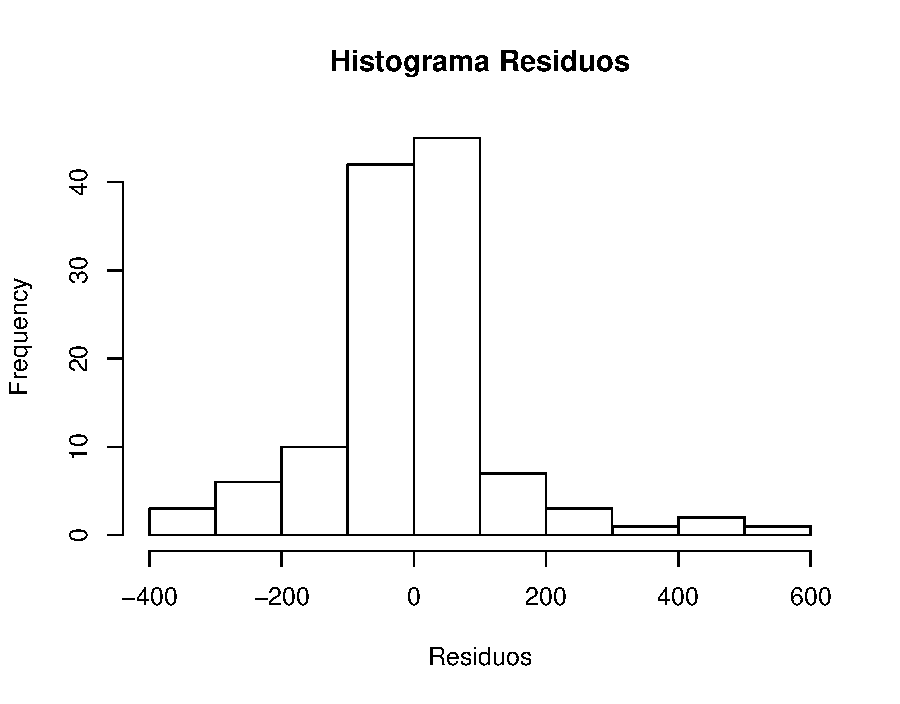
\includegraphics[width=\maxwidth]{figure/unnamed-chunk-16-26} 

}




{\centering 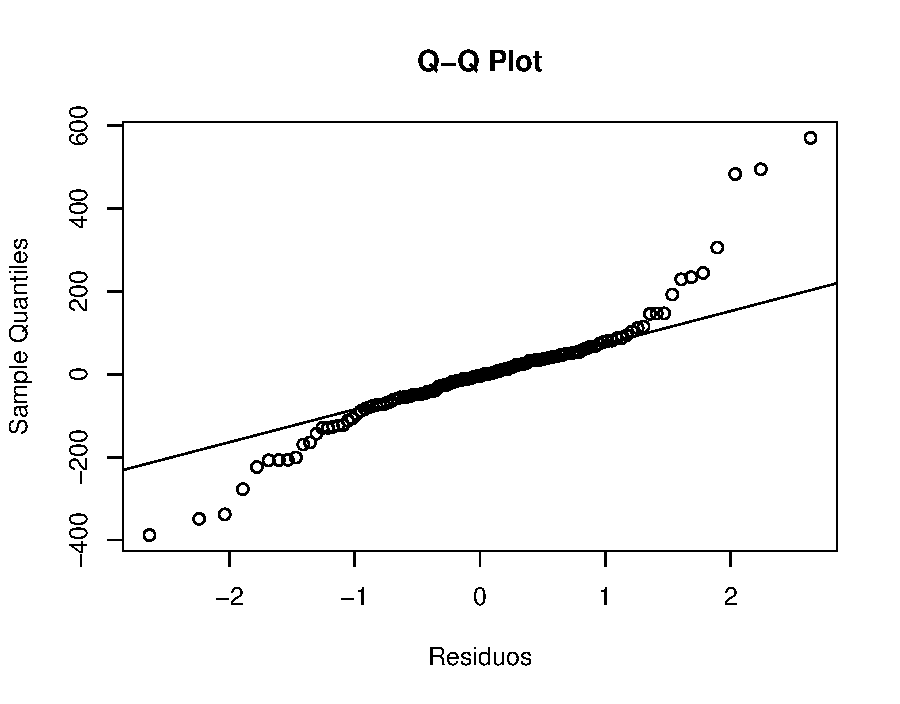
\includegraphics[width=\maxwidth]{figure/unnamed-chunk-16-27} 

}




{\centering 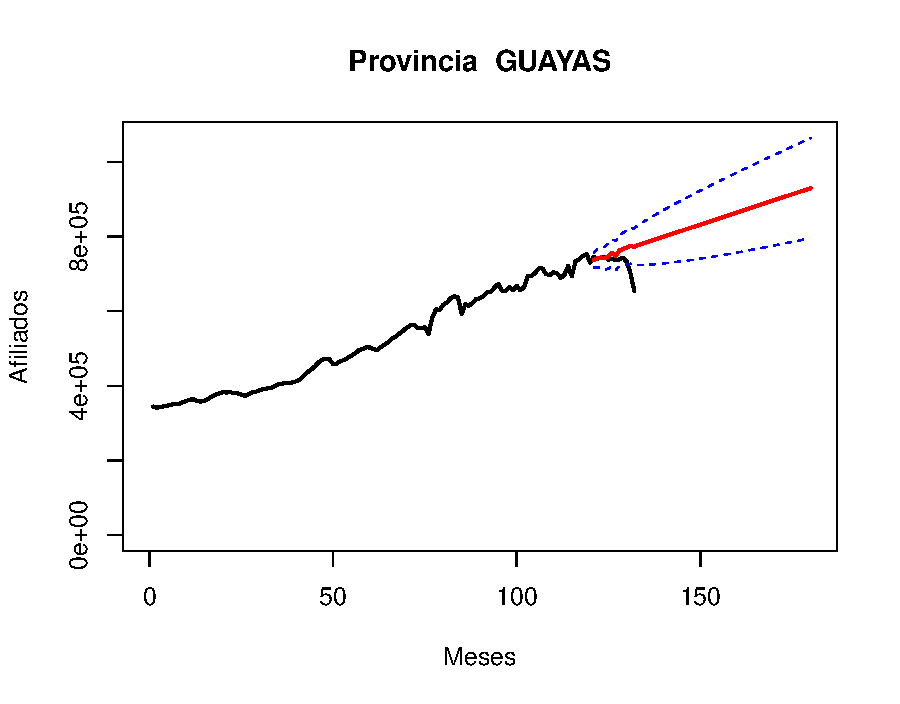
\includegraphics[width=\maxwidth]{figure/unnamed-chunk-16-28} 

}


\begin{kframe}\begin{verbatim}
## Series: data[, i] 
## ARIMA(0,1,1)(0,0,1)[12] with drift         
## 
## Coefficients:
##           ma1    sma1      drift
##       -0.2913  0.2949  3249.9255
## s.e.   0.0962  0.1032   821.4847
## 
## sigma^2 estimated as 98937829:  log likelihood=-1264.84
## AIC=2537.68   AICc=2538.03   BIC=2548.79
\end{verbatim}
\end{kframe}

{\centering 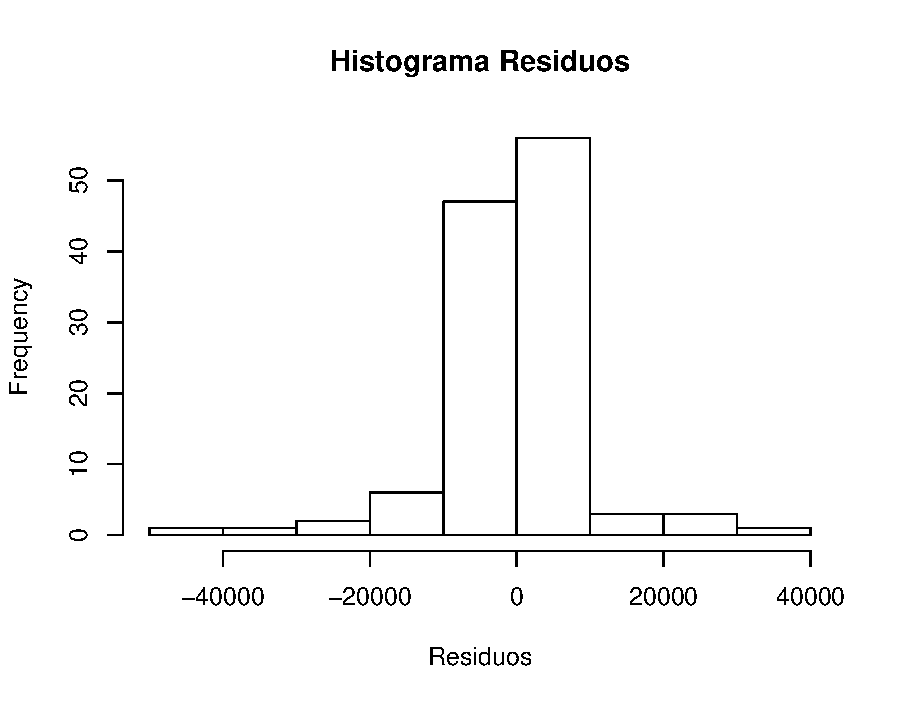
\includegraphics[width=\maxwidth]{figure/unnamed-chunk-16-29} 

}




{\centering 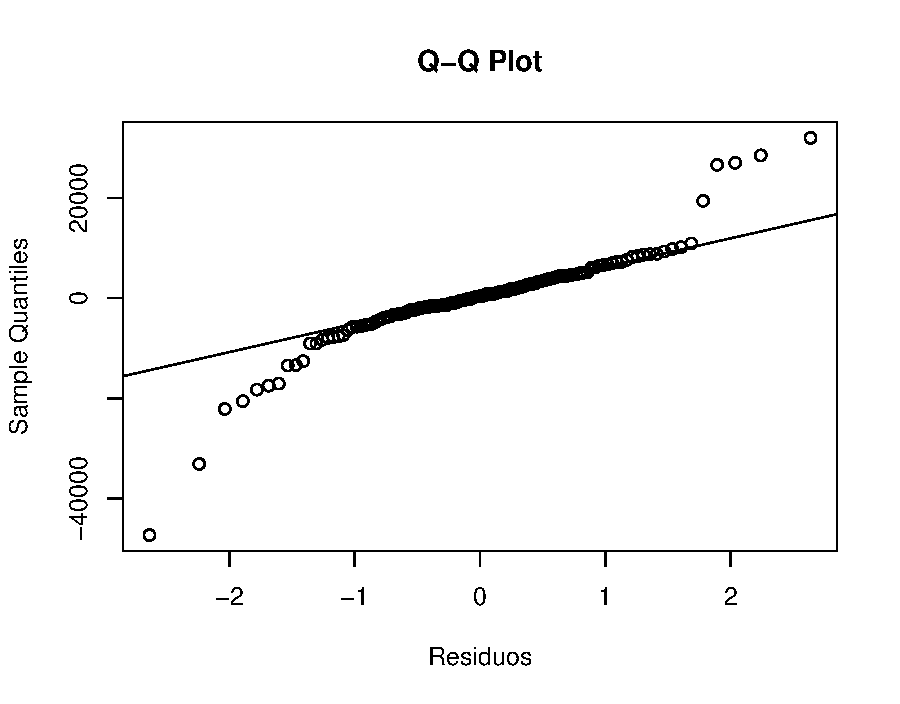
\includegraphics[width=\maxwidth]{figure/unnamed-chunk-16-30} 

}




{\centering 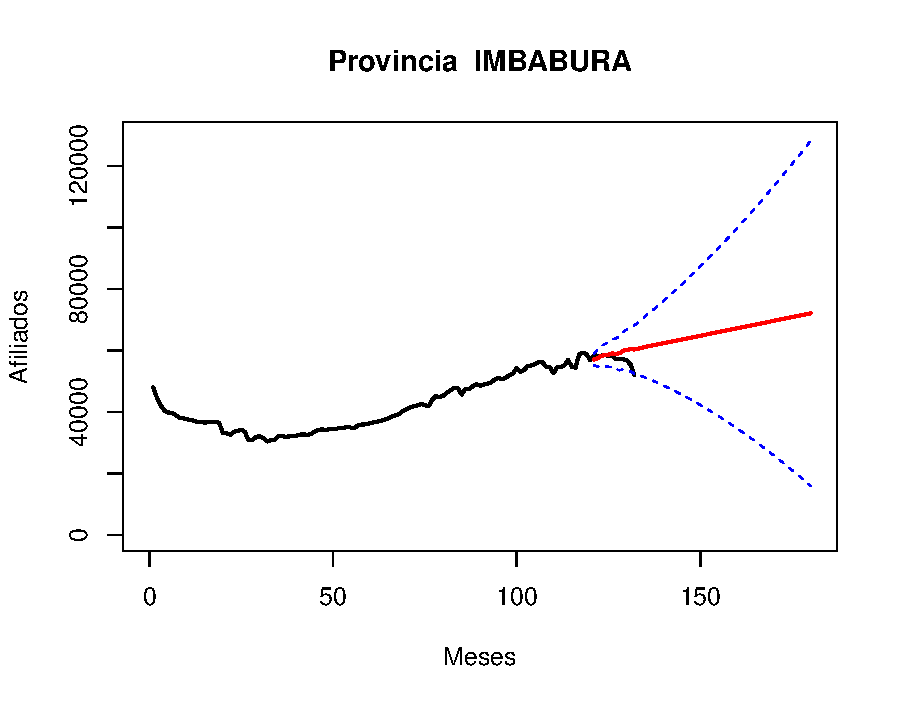
\includegraphics[width=\maxwidth]{figure/unnamed-chunk-16-31} 

}


\begin{kframe}\begin{verbatim}
## Series: data[, i] 
## ARIMA(3,2,2)(0,0,1)[12]                    
## 
## Coefficients:
##          ar1      ar2      ar3      ma1     ma2    sma1
##       0.3792  -0.2286  -0.0757  -1.3271  0.4057  0.1456
## s.e.  0.3454   0.1043   0.1443   0.3338  0.2950  0.1346
## 
## sigma^2 estimated as 906215:  log likelihood=-978.02
## AIC=1970.05   AICc=1971.06   BIC=1989.44
\end{verbatim}
\end{kframe}

{\centering 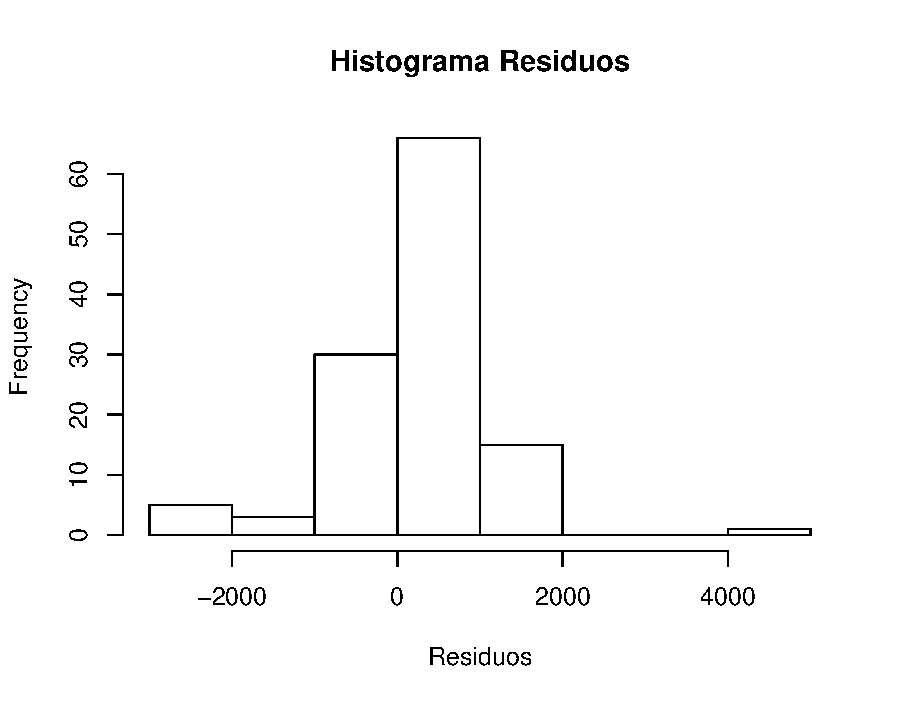
\includegraphics[width=\maxwidth]{figure/unnamed-chunk-16-32} 

}




{\centering 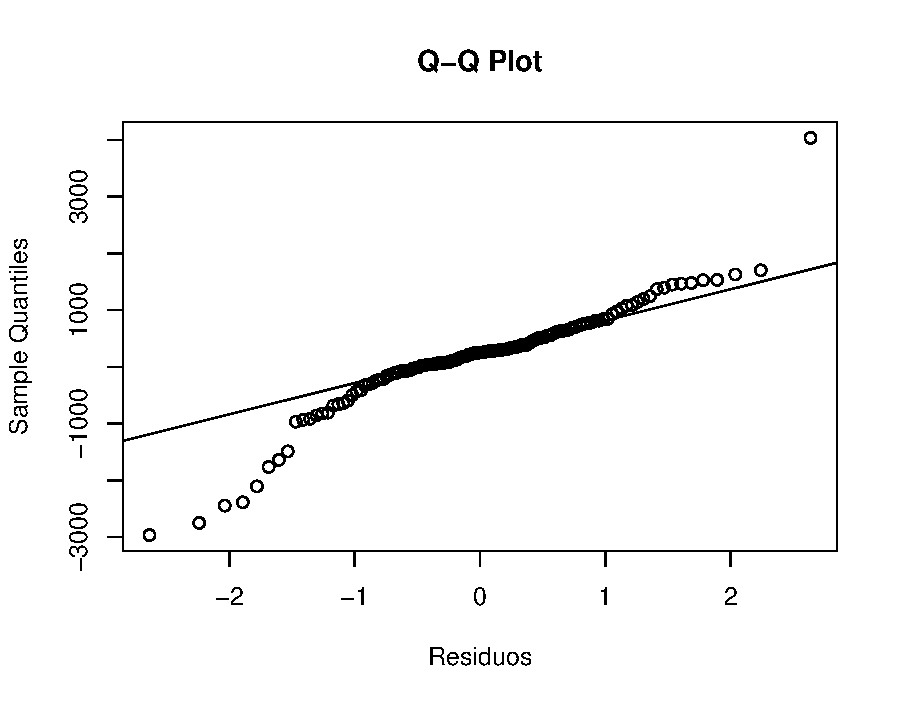
\includegraphics[width=\maxwidth]{figure/unnamed-chunk-16-33} 

}




{\centering 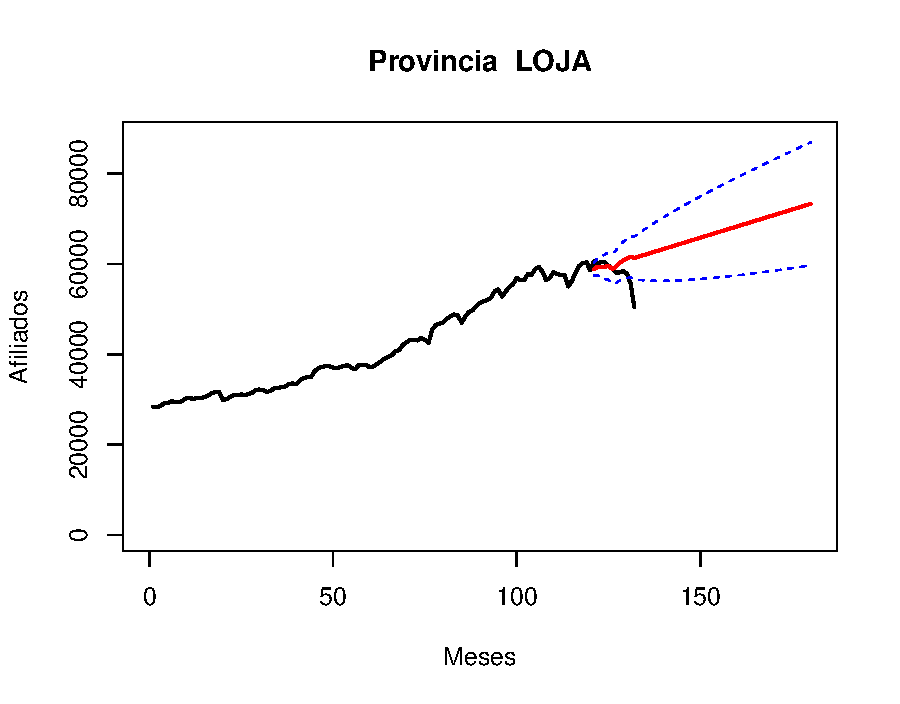
\includegraphics[width=\maxwidth]{figure/unnamed-chunk-16-34} 

}


\begin{kframe}\begin{verbatim}
## Series: data[, i] 
## ARIMA(0,1,0)(0,0,1)[12] with drift         
## 
## Coefficients:
##         sma1     drift
##       0.3438  249.5408
## s.e.  0.0923   83.9328
## 
## sigma^2 estimated as 488130:  log likelihood=-948.96
## AIC=1903.92   AICc=1904.13   BIC=1912.26
\end{verbatim}
\end{kframe}

{\centering 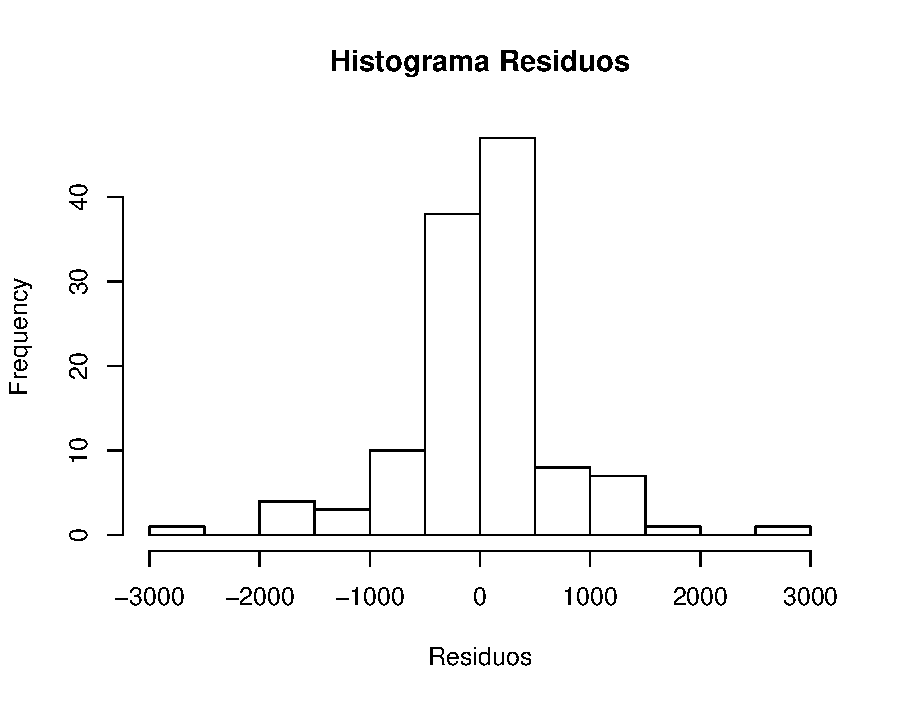
\includegraphics[width=\maxwidth]{figure/unnamed-chunk-16-35} 

}




{\centering 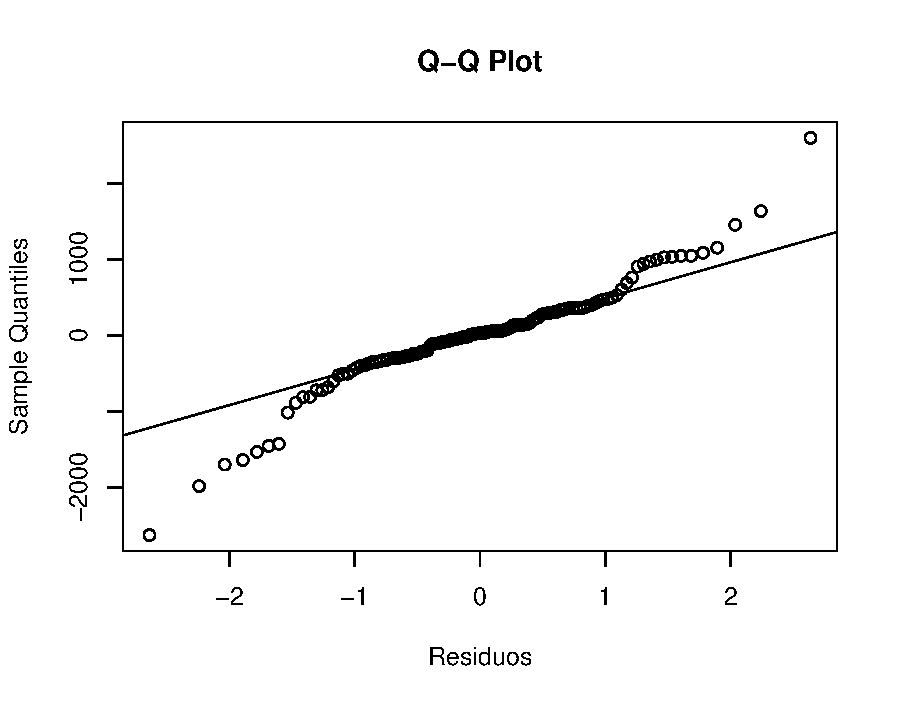
\includegraphics[width=\maxwidth]{figure/unnamed-chunk-16-36} 

}




{\centering 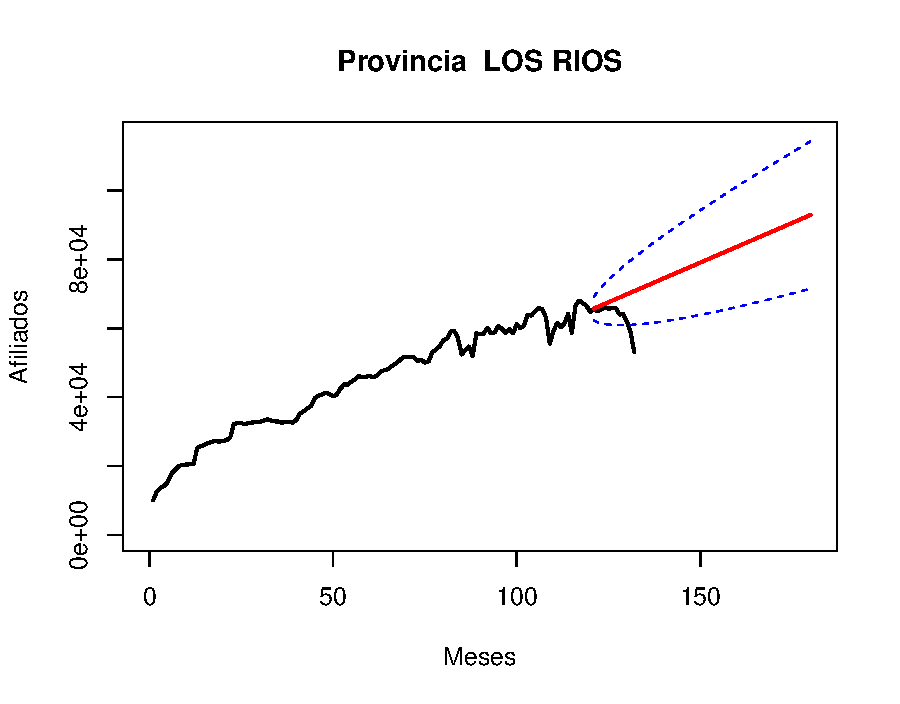
\includegraphics[width=\maxwidth]{figure/unnamed-chunk-16-37} 

}


\begin{kframe}\begin{verbatim}
## Series: data[, i] 
## ARIMA(0,1,1) with drift         
## 
## Coefficients:
##           ma1     drift
##       -0.2029  459.9023
## s.e.   0.0977  128.6499
## 
## sigma^2 estimated as 3086349:  log likelihood=-1057.95
## AIC=2121.91   AICc=2122.12   BIC=2130.24
\end{verbatim}
\end{kframe}

{\centering 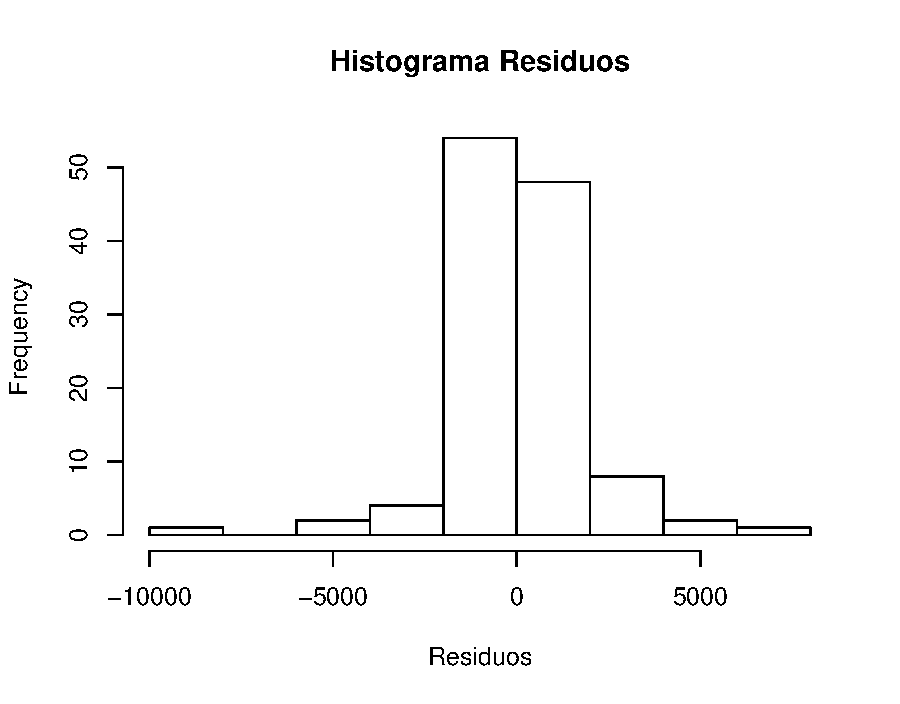
\includegraphics[width=\maxwidth]{figure/unnamed-chunk-16-38} 

}




{\centering \includegraphics[width=\maxwidth]{figure/unnamed-chunk-16-39} 

}




{\centering \includegraphics[width=\maxwidth]{figure/unnamed-chunk-16-40} 

}


\begin{kframe}\begin{verbatim}
## Series: data[, i] 
## ARIMA(2,1,0)(1,0,1)[12] with drift         
## 
## Coefficients:
##           ar1      ar2    sar1     sma1     drift
##       -0.3627  -0.1184  0.7409  -0.3345  836.3650
## s.e.   0.0976   0.0942  0.1345   0.1844  213.9424
## 
## sigma^2 estimated as 2644289:  log likelihood=-1050.87
## AIC=2113.75   AICc=2114.5   BIC=2130.42
\end{verbatim}
\end{kframe}

{\centering \includegraphics[width=\maxwidth]{figure/unnamed-chunk-16-41} 

}




{\centering \includegraphics[width=\maxwidth]{figure/unnamed-chunk-16-42} 

}




{\centering \includegraphics[width=\maxwidth]{figure/unnamed-chunk-16-43} 

}


\begin{kframe}\begin{verbatim}
## Series: data[, i] 
## ARIMA(0,1,1)(0,0,2)[12] with drift         
## 
## Coefficients:
##           ma1    sma1    sma2    drift
##       -0.3558  0.2654  0.2249  66.8423
## s.e.   0.0950  0.1185  0.1262  28.6697
## 
## sigma^2 estimated as 115319:  log likelihood=-863.33
## AIC=1736.66   AICc=1737.2   BIC=1750.56
\end{verbatim}
\end{kframe}

{\centering \includegraphics[width=\maxwidth]{figure/unnamed-chunk-16-44} 

}




{\centering \includegraphics[width=\maxwidth]{figure/unnamed-chunk-16-45} 

}




{\centering \includegraphics[width=\maxwidth]{figure/unnamed-chunk-16-46} 

}


\begin{kframe}\begin{verbatim}
## Series: data[, i] 
## ARIMA(1,1,0)(0,0,1)[12] with drift         
## 
## Coefficients:
##           ar1    sma1    drift
##       -0.4089  0.2191  58.9439
## s.e.   0.0833  0.1059  26.0632
## 
## sigma^2 estimated as 110432:  log likelihood=-860.16
## AIC=1728.33   AICc=1728.68   BIC=1739.44
\end{verbatim}
\end{kframe}

{\centering \includegraphics[width=\maxwidth]{figure/unnamed-chunk-16-47} 

}




{\centering \includegraphics[width=\maxwidth]{figure/unnamed-chunk-16-48} 

}




{\centering \includegraphics[width=\maxwidth]{figure/unnamed-chunk-16-49} 

}


\begin{kframe}\begin{verbatim}
## Series: data[, i] 
## ARIMA(1,1,2)(0,0,1)[12] with drift         
## 
## Coefficients:
##           ar1     ma1      ma2    sma1     drift
##       -0.5778  0.5061  -0.4189  0.2924  140.2573
## s.e.   0.1183  0.1450   0.1269  0.1349   36.9276
## 
## sigma^2 estimated as 210776:  log likelihood=-898.24
## AIC=1795.96   AICc=1796.71   BIC=1812.63
\end{verbatim}
\end{kframe}

{\centering \includegraphics[width=\maxwidth]{figure/unnamed-chunk-16-50} 

}




{\centering \includegraphics[width=\maxwidth]{figure/unnamed-chunk-16-51} 

}




{\centering \includegraphics[width=\maxwidth]{figure/unnamed-chunk-16-52} 

}


\begin{kframe}\begin{verbatim}
## Series: data[, i] 
## ARIMA(0,1,1)(0,0,1)[12] with drift         
## 
## Coefficients:
##           ma1    sma1    drift
##       -0.5429  0.3556  51.5353
## s.e.   0.0761  0.1051  11.7900
## 
## sigma^2 estimated as 44455:  log likelihood=-806.62
## AIC=1621.25   AICc=1621.6   BIC=1632.36
\end{verbatim}
\end{kframe}

{\centering \includegraphics[width=\maxwidth]{figure/unnamed-chunk-16-53} 

}




{\centering \includegraphics[width=\maxwidth]{figure/unnamed-chunk-16-54} 

}




{\centering \includegraphics[width=\maxwidth]{figure/unnamed-chunk-16-55} 

}


\begin{kframe}\begin{verbatim}
## Series: data[, i] 
## ARIMA(1,1,2)(0,0,2)[12] with drift         
## 
## Coefficients:
##           ar1     ma1      ma2    sma1    sma2      drift
##       -0.8265  0.6085  -0.3601  0.2209  0.1534  4313.3934
## s.e.   0.0708  0.1030   0.0948  0.1022  0.0890   786.5182
## 
## sigma^2 estimated as 88992256:  log likelihood=-1258.76
## AIC=2531.51   AICc=2532.52   BIC=2550.97
\end{verbatim}
\end{kframe}

{\centering \includegraphics[width=\maxwidth]{figure/unnamed-chunk-16-56} 

}




{\centering \includegraphics[width=\maxwidth]{figure/unnamed-chunk-16-57} 

}




{\centering \includegraphics[width=\maxwidth]{figure/unnamed-chunk-16-58} 

}


\begin{kframe}\begin{verbatim}
## Series: data[, i] 
## ARIMA(1,1,0) with drift         
## 
## Coefficients:
##           ar1     drift
##       -0.1600  203.9975
## s.e.   0.0907   66.8343
## 
## sigma^2 estimated as 713469:  log likelihood=-970.8
## AIC=1947.6   AICc=1947.81   BIC=1955.94
\end{verbatim}
\end{kframe}

{\centering \includegraphics[width=\maxwidth]{figure/unnamed-chunk-16-59} 

}




{\centering \includegraphics[width=\maxwidth]{figure/unnamed-chunk-16-60} 

}




{\centering \includegraphics[width=\maxwidth]{figure/unnamed-chunk-16-61} 

}


\begin{kframe}\begin{verbatim}
## Series: data[, i] 
## ARIMA(0,1,0) with drift         
## 
## Coefficients:
##          drift
##       389.6050
## s.e.  171.0239
## 
## sigma^2 estimated as 3480649:  log likelihood=-1065.09
## AIC=2134.17   AICc=2134.28   BIC=2139.73
\end{verbatim}
\end{kframe}

{\centering \includegraphics[width=\maxwidth]{figure/unnamed-chunk-16-62} 

}




{\centering \includegraphics[width=\maxwidth]{figure/unnamed-chunk-16-63} 

}




{\centering \includegraphics[width=\maxwidth]{figure/unnamed-chunk-16-64} 

}


\begin{kframe}\begin{verbatim}
## Series: data[, i] 
## ARIMA(2,2,1)(0,0,2)[12]                    
## 
## Coefficients:
##           ar1      ar2      ma1    sma1    sma2
##       -0.3800  -0.1534  -0.9225  0.1800  0.2587
## s.e.   0.1086   0.1041   0.0469  0.1186  0.1428
## 
## sigma^2 estimated as 195494:  log likelihood=-888.53
## AIC=1789.06   AICc=1789.82   BIC=1805.68
\end{verbatim}
\end{kframe}

{\centering \includegraphics[width=\maxwidth]{figure/unnamed-chunk-16-65} 

}




{\centering \includegraphics[width=\maxwidth]{figure/unnamed-chunk-16-66} 

}




{\centering \includegraphics[width=\maxwidth]{figure/unnamed-chunk-16-67} 

}


\begin{kframe}\begin{verbatim}
## Series: data[, i] 
## ARIMA(0,1,0)(0,0,1)[12] with drift         
## 
## Coefficients:
##         sma1     drift
##       0.1360  399.5611
## s.e.  0.1007  101.7942
## 
## sigma^2 estimated as 976849:  log likelihood=-989.59
## AIC=1985.19   AICc=1985.4   BIC=1993.53
\end{verbatim}
\end{kframe}

{\centering \includegraphics[width=\maxwidth]{figure/unnamed-chunk-16-68} 

}




{\centering \includegraphics[width=\maxwidth]{figure/unnamed-chunk-16-69} 

}




{\centering \includegraphics[width=\maxwidth]{figure/unnamed-chunk-16-70} 

}


\begin{kframe}\begin{verbatim}
## Series: data[, i] 
## ARIMA(1,1,1)(0,0,1)[12] with drift         
## 
## Coefficients:
##          ar1      ma1    sma1    drift
##       0.3897  -0.7511  0.5025  79.4536
## s.e.  0.1594   0.1111  0.1033  18.3544
## 
## sigma^2 estimated as 109130:  log likelihood=-860.95
## AIC=1731.9   AICc=1732.44   BIC=1745.8
\end{verbatim}
\end{kframe}

{\centering \includegraphics[width=\maxwidth]{figure/unnamed-chunk-16-71} 

}




{\centering \includegraphics[width=\maxwidth]{figure/unnamed-chunk-16-72} 

}



\end{knitrout}

kable(matrix(rnorm(40), 5))


\end{document}
